% ===================================================================
% FST-III: Biological Stability and Nash Frustration
% Target: Journal of Theoretical Biology / BioSystems
% Version: 1.7 (R119 corrective follow-up, 2026-10-01; not a new biological validation)
% ===================================================================

\documentclass[12pt,a4paper]{article}

% Packages
\usepackage[utf8]{inputenc}
\usepackage[T1]{fontenc}
\usepackage{lmodern}
\input{glyphtounicode}
\pdfgentounicode=1
\usepackage[english]{babel}
\usepackage{amsmath,amssymb,amsthm}
\usepackage{physics}
\usepackage{graphicx}
\usepackage{booktabs}
\usepackage{tabularx}
\usepackage{array}
\usepackage[margin=2.5cm]{geometry}
\usepackage{natbib}
\usepackage{enumitem}
\usepackage{microtype}
\usepackage{xurl}
\usepackage[unicode=true]{hyperref}
\usepackage{cleveref}
\usepackage{tikz}
\usetikzlibrary{arrows.meta,positioning,calc,fit,backgrounds}

\graphicspath{{../results/}{../fst_nash/results/}}
\setlength{\emergencystretch}{3em}
\newcolumntype{L}[1]{>{\raggedright\arraybackslash\hspace{0pt}}p{#1}}
\newcolumntype{Y}{>{\raggedright\arraybackslash\hspace{0pt}}X}
\makeatletter
\renewcommand*{\HyperDestNameFilter}[1]{en.#1}
\makeatother

% Theorem environments
\newtheorem{proposition}{Proposition}
\newtheorem{conjecture}{Conjecture}
\newtheorem{hypothesis}{Hypothesis}
\newtheorem{definition}{Definition}
\theoremstyle{remark}
\newtheorem{remark}{Remark}

% Title
\title{Functional Stability Theory III: Biological Stability and Nash Frustration}

\author{Lukas Geiger\\
\textit{Independent Researcher, Bernau, Germany}\\
ORCID: \url{https://orcid.org/0009-0005-7296-1534}}

\date{October 2026 --- corrective version 1.7}

\hypersetup{
  pdftitle={Functional Stability Theory III: Biological Stability and Nash Frustration},
  pdfauthor={Lukas Geiger},
  pdfsubject={Biological stability across scales in Functional Stability Theory},
  pdfkeywords={evolutionary game theory, protein folding, gene regulation, dissipative adaptation, Free Energy Principle, MEPP, Boolean networks}
}

\begin{document}

\maketitle
\begin{abstract}
This paper develops a conjectural framework for biological organization spanning molecular to ecosystem scales, organized around thermodynamic game theory and the Maximum Entropy Production Principle (MEPP). It examines whether biological stability problems can be modeled as dissipative structures whose attractors admit Nash-style fixed-point descriptions once players, strategies, and payoffs are specified at the relevant scale. The framework brings England's dissipative adaptation theory, Friston's Free Energy Principle, Kauffman's Boolean network dynamics, and classical evolutionary game theory into a working hierarchy: at each level---from protein folding through gene regulation, cellular coalitions, to ecosystem dynamics---game-theoretic stability offers a common language for biological organization. The major evolutionary transitions are treated as possible coarse-graining steps that may preserve this structure across scales. As a concrete application, we introduce \emph{Nash frustration} for protein structures and provide a preliminary single-protein consistency test against NMR chemical shift perturbation data (Spearman rank correlation $\rho_S = 0.44$, $p = 0.033$, $n = 24$). The normalized residue ranking is independent of~$\eta$ in the checked local scan window, while absolute instability scales, including $\rho(J)$, remain calibration targets. This score is not a Nash or kinetic stability certificate; MFG existence, uniqueness, and convergence require separate assumptions. The framework proposes testable hypotheses for protein folding landscapes, gene regulatory network attractors, and ecosystem resilience.
\end{abstract}

\textbf{Keywords:} evolutionary game theory, ESS, protein folding, gene regulation, MEPP, dissipative adaptation, Free Energy Principle, Boolean networks, major transitions, coarse-graining

\clearpage
\tableofcontents
\clearpage

% ===================================================================
\section{Introduction}
\label{sec:introduction}
% ===================================================================

The emergence and stabilization of biological complexity presents modern science with the challenge of bridging the fundamental laws of physics and the dynamic strategies of life. The Functional Stability Theory (FST-III) framework treats biological systems not merely as products of random mutations but as candidate dissipative structures operating within thermodynamic constraints~\citep{EcosystemMEPP}.

This paper investigates the proposed connection between game theory and the Maximum Entropy Production Principle (MEPP), exploring whether biological stability can be understood through the lens of game-theoretic attractors within thermodynamic constraints. The scope is primarily biological (Sections~\ref{sec:thermodynamics}--\ref{sec:ecosystem}); cosmological extensions are briefly noted in Section~\ref{sec:cosmology} but are not part of the core argument.

Classical evolutionary game theory, pioneered by \citet{MaynardSmithPrice1973} and \citet{MaynardSmith1982}, revolutionized our understanding of biological behavior. Yet the standard treatment is largely confined to behavioral ecology. This paper explores a broader proposal: game-theoretic descriptions may be formulated at multiple levels of biological organization, and these descriptions connect biology to physics through an analogous stability logic developed in FST-I~\citep{FSTI} and FST-II~\citep{FSTII}.

% ===================================================================
\section{Structural Alignment: FST-III as a Pattern A Instance}
\label{sec:structural-alignment}
% ===================================================================

The biological stability framework developed here (ESS/FEP) is proposed as a \textbf{Pattern-A-style structural analogy} within the FST ecosystem (see~\citealp{FST-Unified2026}), not as a formal derivation from the mathematical Pattern A program. The recent \textbf{gauge-theoretic reformulation of the Riemann Hypothesis} (see~\citealp{GeigerRH2026c}) provides a motivating structural template for this architecture.

Within this hierarchical stability framework, biological systems are understood as follows:
\begin{enumerate}[label=\alph*)]
    \item \textbf{Analytical Rank-Finiteness (Null-Tail):} Biological complexity may be constrained against the combinatorial explosion of the ``dead'' state because, at any given environmental boundary condition, only a limited set of genotype configurations may satisfy simultaneous ESS and FEP stability. This finiteness is conjectured, not proven; it is motivated by the observation that the intersection of ESS conditions (stability against invasion) and thermodynamic viability (positive dissipation) imposes sufficiently many independent constraints to reduce the solution set to a discrete collection. The unorganized ``noise'' is filtered by the entropic constraint, supporting robust persistence.
    \item \textbf{Finite Negativity as Gauge-Signal (Structural Analogy):} Genetic conflict, cancer, and competition play a role analogous to finite negativity in the arithmetical kernel. They are not treated here as random defects, but as signals of incomplete organizational coordination that can be reduced or reorganized through new levels of cooperation (major transitions). This analogy is structural, not formal: the mathematical mechanisms differ, but the logical pattern (destabilization signals driving reorganization) is shared.
    \item \textbf{Constrained Functional Positivity (Biological Attractors):} The stable attractors of a gene network or ecosystem may be represented as ``gauge-stable'' states where the free-energy functional reaches a constrained minimum. In analogy with rank-reduction mechanisms in the RH program, phenotypic stability is interpreted here as the result of a finite set of epigenetic constraints supporting thermodynamic viability.
\end{enumerate}

This alignment frames FST-III as a structural analogy---not a formal derivation---to ``Functional Positivity under Constraint.''

\begin{definition}[Resolvent-stable fixed point]
\label{def:resolvent-stable}
A fixed point of a dynamical system is called \emph{resolvent-stable} if second-order perturbation analysis (Hessian eigenvalues or resolvent expansion coefficients) yields strictly positive values in all non-gauge directions---i.e., all perturbation modes orthogonal to symmetry-generated degeneracies are stabilized. In biological systems, ``non-gauge directions'' correspond to perturbation modes that change observable phenotypic properties (e.g., protein conformation, gene expression pattern), while ``gauge directions'' correspond to neutral degrees of freedom that leave the phenotype invariant (e.g., synonymous codon substitutions, neutral conformational fluctuations within a basin). This is a structural analogy---motivated by, but not formally derived from---the spectral gap property established in the FST-RH framework~\citep{GeigerRH2026b}; its application to biological systems requires domain-specific verification of which directions are genuinely ``gauge.''
\end{definition}

% ===================================================================
\section{Thermodynamic Foundations: MEPP and Dissipative Adaptation}
\label{sec:thermodynamics}
% ===================================================================

\subsection{Life as Non-Equilibrium Phenomenon}

The classification of biological processes in thermodynamics begins with the recognition that life is a phenomenon far from thermodynamic equilibrium~\citep{EcosystemMEPP}. While closed systems inevitably tend toward the state of maximum entropy and heat death, biological systems maintain themselves through continuous export of entropy to their environment---a process that Erwin Schrödinger described in 1944 as the acquisition of ``negentropy''~\citep{SchoolBiologicalPhysics,EcosystemMEPP,Kuzu2025}.

\subsection{Three Thermodynamic Hypotheses}

Within the FST-III framework, three central thermodynamic hypotheses describe the behavior of living matter~\citep{EcosystemMEPP}:

\begin{enumerate}
    \item \textbf{Thermodynamic Fingerprint of Life:} Living communities significantly increase the rate of entropy production compared to abiotic counterparts under identical boundary conditions.

    \item \textbf{State Selection Principle (Stability Interpretation):} When a system can reach multiple stable states, the resolvent-stable configuration---where second-order destabilization channels are suppressed---tends to exhibit high (though not necessarily maximal) entropy production rates.

    \item \textbf{Gradient Response Principle:} When the external thermodynamic gradient increases, the system transitions to a new stable state characterized by even higher entropy production.
\end{enumerate}

\begin{table}[htbp]
\centering
\caption{Thermodynamic principles and their biological relevance. MEPP applies to strongly driven systems; Prigogine's minimum entropy production holds only near equilibrium.}
\label{tab:thermo-principles}
\begin{tabularx}{\textwidth}{@{}L{0.21\textwidth} L{0.28\textwidth} Y@{}}
\toprule
\textbf{Principle} & \textbf{Description} & \textbf{Biological Relevance} \\
\midrule
MEPP & Stability filter favoring high dissipation & Metabolic efficiency selection \\
State Selection & Stability correlates with high $\dot{S}$ & Complex food web stabilization \\
Gradient Response & Adaptation to increasing energy input & Photosynthetic efficiency increase \\
Prigogine (LMEP) & Minimal entropy near equilibrium & Only for linear, weakly driven systems \\
\bottomrule
\end{tabularx}
\end{table}

\begin{remark}[MEPP as Stability Filter, not Selection Law]
\label{rem:mepp-stability-biology}
Following the resolvent analysis from the Riemann Hypothesis program~\citep{GeigerRH2026b}, the three thermodynamic hypotheses above are read here as \emph{stability filters} rather than selection laws. The key distinctions are:
\begin{enumerate}[label=(\roman*)]
  \item \textbf{Not a causal driver:} MEPP does not causally drive biological systems toward states of maximum entropy production.
  \item \textbf{Degeneracy at leading order:} Many biological configurations are viable at first order; the leading-order dynamics are degenerate.
  \item \textbf{Second-order filter:} MEPP acts as a second-order filter that eliminates resolvent-unstable configurations---those susceptible to perturbation-induced collapse via cross-coupling between metabolic, structural, and replicative degrees of freedom.
  \item \textbf{Candidate fixed point:} The state with ``highest entropy production'' is more cautiously read as a candidate resolvent-stable fixed point within the degenerate manifold of thermodynamically viable configurations.
\end{enumerate}
This refinement addresses the criticism that MEPP is used as a selection law: it is a stability criterion, not a causal driver. For the full development in the prebiotic context, including the formal England inequality and the MEPP controversy, see FST-II~\citep{FSTII}; here we apply this principle specifically to biological systems.
\end{remark}

\subsection{Dissipative Adaptation: The Physics of Self-Organization}

A crucial link between pure thermodynamics and biological structure is provided by Jeremy England's theory of dissipative adaptation~\citep{England2013,EnglandNano}. For the full formal derivation of England's dissipation bound from the Crooks fluctuation theorem, the game-theoretic reading of the inequality, and the causal-direction caveat, see FST-II~\citep{FSTII}; here we summarize only the aspects relevant to the biological context.

\citet{England2013} argues, based on non-equilibrium statistics, that matter exposed to a strong external energy source tends to organize itself into configurations that are particularly good at absorbing energy and dissipating it as heat.

The mechanism of dissipative adaptation relies on the irreversibility of state transitions. When a system absorbs energy from an external source, it can overcome energetic activation barriers that would be impassable through purely thermal fluctuations. Once this energy is dissipated, the system lacks the energy to jump back to the initial state. Over time, structures accumulate that exhibit high resonance with the external energy source~\citep{EnglandNano}.

This process offers one physical account of the spontaneous emergence of self-replicating structures: replication is a direct route by which a system can increase its capacity for energy absorption and dissipation~\citep{EnglandNano}. In this context, ``fitness'' appears not as a purely biological concept but as a physical property of structural persistence under energetic drive~\citep{England2013}.

% ===================================================================
\section{Game-Theoretic Stability: Molecular ESS}
\label{sec:molecular}
% ===================================================================

Once physical structures cross the threshold to biological reproduction, their interactions can be represented with game-theoretic rules.

\subsection{Nash Equilibrium and ESS}

The central concept is the Nash equilibrium, defined by John Nash in 1950, describing states where no actor can improve their payoff through unilateral change of their strategy~\citep{NashPNAS,NashSFI}. In biology, John Maynard Smith and George Price developed this into the Evolutionarily Stable Strategy (ESS)~\citep{MaynardSmithPrice1973,MaynardSmith1982}.

\begin{definition}[Evolutionarily Stable Strategy]
An ESS is a strategy that, when adopted by most members of a population, cannot be invaded by a rare mutant strategy. Every ESS is a Nash equilibrium, but not every Nash equilibrium is an ESS, since ESS requires additional stability conditions against invasions~\citep{MaynardSmith1982}.
\end{definition}

In FST-III, this principle is transferred to the molecular level. Proteins, enzymes, and regulatory RNAs are considered ``players'' whose ``strategies'' consist of their structural configurations and catalytic activities~\citep{GameBiochemistry}.

\begin{remark}[ESS as Resolvent-Stable Fixed Point]
\label{rem:ess-resolvent}
A proposed lesson from the resolvent analysis of the Riemann Hypothesis~\citep{GeigerRH2026b} refines the interpretation of ESS. An ESS need not be read as a global fitness optimum; in this analogy, it is a resolvent-stable fixed point. At leading order, the fitness landscape may be degenerate---many phenotypic configurations yield comparable payoffs. Selection then acts at second order through resolvent-type couplings between the degenerate modes: invasion dynamics, frequency-dependent interactions, and spatial coupling collectively split the degeneracy. The ESS is the candidate configuration where second-order destabilization channels are jointly suppressed. Nash frustration (defined below in Section~\ref{sec:molecular}) is therefore not simply a defect but a possible structural feature of this resolvent architecture: it reflects residual second-order coupling that may stabilize the configuration while preventing crystallization into a rigid, fragile optimum.
\end{remark}

\begin{table}[htbp]
\centering
\caption{Mapping of game-theoretic concepts to physical and biological counterparts.}
\label{tab:game-biology-mapping}
\begin{tabularx}{\textwidth}{@{}L{0.18\textwidth} L{0.29\textwidth} Y@{}}
\toprule
\textbf{Game Concept} & \textbf{Physical Correspondence} & \textbf{Biological Example} \\
\midrule
Nash Equilibrium & No profitable unilateral deviation & Conditional game-model description \\
ESS & Attractor with local stability & Allele fixation \\
Payoff Matrix & Energy/fitness landscape & Enzyme-substrate affinity \\
Mixed Strategy & Population heterogeneity & Division of labor in colonies \\
Nash Frustration & Step-dependent surrogate spectral excess & Unvalidated protein-function hypothesis \\
\bottomrule
\end{tabularx}
\end{table}

\subsection{Protein Folding as an Optimization Game}

Protein folding can be modeled heuristically as a game against a thermodynamic landscape~\citep{EnzymeFolding}. The native conformation is a candidate, rather than a certified equilibrium, in an $n$-player model with the following choices:

\begin{itemize}
    \item \textbf{Players:} Individual amino acid residues
    \item \textbf{Strategies:} Backbone dihedral angles $(\phi, \psi)$
    \item \textbf{Payoff:} $-\Delta G$ (negative free energy change)
    \item \textbf{Equilibrium candidate:} Native conformation; Anfinsen's thermodynamic hypothesis alone does not certify unilateral optimality for the fitted model~\citep{Anfinsen1973}
\end{itemize}

Misfolded proteins and prions motivate metastability questions, but kinetic trapping or template-directed propagation does not by itself establish a local Nash equilibrium. That classification requires the specified payoff and permitted unilateral deviations to be checked. The present fitted torsion model supplies no such certification for prion propagation.

\subsection{Nash Frustration vs.\ Energetic Frustration}

\paragraph{Corrective scope (version 1.7).}
This follow-up corrects two inventory findings: the Hessian-derived gradient surrogate does not certify Nash status, and MFG existence is distinct from monotonicity-based uniqueness and algorithmic convergence. Historical numerical values are retained as exploratory model outputs, without new computation or biological validation. Previously proposed unrestricted \emph{proof repairs} are not accepted; native HP35 stationarity, the actual sequential-sweep derivative, the protein-specific MFG regularity contract, and a full claim/source review remain open.

\paragraph{Local versus global unilateral optimality.}
For a $C^2$ shared cost at an interior stationary point, each player's own Hessian block being positive definite suffices for strict local Nash status; positive semidefiniteness is necessary, not sufficient. Positive definiteness is not necessary. These are unilateral tests, not positivity of the collective Hessian, and they do not certify global best responses~\citep{RatliffBurdenSastry2016}. With coordinate order $(\phi_1,\ldots,\phi_N,\psi_1,\ldots,\psi_N)$, residue $i$ uses indices $(i,N+i)$, not adjacent pairs. None of these conditions has been established for the fitted native HP35 state here.




\noindent\textit{Notation:} $\rho(J)$ denotes the spectral radius of the Jacobian, $\rho_S$ the Spearman correlation coefficient, and $\rho_i$ the normalized residue-level frustration score. These distinct uses of $\rho$ follow their respective community conventions and are disambiguated by subscript throughout.

The concept of local frustration in protein structures has been extensively studied through the Protein Frustratometer~\citep{Ferreiro2007,Ferreiro2014} as well as sequence- and proteome-scale deep learning models such as FrustraMPNN~\citep{Beining2026} and FrustrAI-Seq~\citep{Leusch2026}, which identifies residues where the native amino acid identity is suboptimal given the local structural environment. This energetic frustration correlates with functional sites, binding interfaces, and allosteric regions.

The historical name \textbf{Nash frustration} denotes a candidate diagnostic (Table~\ref{tab:frustration-comparison}). Here it asks which residues carry spectral excess of a specified gradient surrogate; it does not establish which residues admit profitable unilateral deviations.

Formally, \emph{residue-level Nash frustration} is computed from $J=I-\eta H$, the derivative of the synchronous gradient map $\theta\mapsto\theta-\eta\nabla F(\theta)$. Here $H$ is the $2n\times2n$ Hessian of the fitted potential and $\eta>0$ a chosen step. This is not the Jacobian of the sequential approximate best-response routine. The score for residue $i$ is:
\begin{equation}
\text{frustration}(i) = \sum_{k: |\lambda_k| > 1} (|\lambda_k| - 1) \left( v_{k,\phi_i}^2 + v_{k,\psi_i}^2 \right)
\end{equation}
where $\lambda_k,v_k$ are eigenpairs of $J$. The spectral radius $\rho(J)=\max_k|\lambda_k|$ and residue projection describe this surrogate only. At a stationary point, $\rho(J)>1$ signals a linearly expanding surrogate mode; away from stationarity it is only a local derivative diagnostic. Negative collective curvature or excessive steps in positive-curvature modes can cause expansion. Neither $\rho(J)>1$ nor proximity to one decides local or global Nash status.

\paragraph{Coordinate-metric caveat.}
The projection above uses the Euclidean norm of eigenvector components in the local dihedral chart $(\phi,\psi)$. It is therefore a chart-level diagnostic, not an intrinsic coordinate-invariant biomolecular observable. An intrinsic or mass-weighted version should replace the squared component sum by a metric-weighted projection using the appropriate torsional/manifold metric; the present single-protein benchmark uses a fixed chart and should be interpreted under that convention.

\paragraph{Preliminary consistency check and $\eta$-independence.}
We performed a preliminary single-protein consistency check of the Nash-frustration ranking against experimental NMR chemical shift perturbation (CSP) data derived from BMRB entry~4428~\citep{BMRB4428}. This BMRB entry is the HP67 villin-headpiece NMR data set (primary PDB 1QQV); for the HP35 structural benchmark (PDB 1YRF), we used the documented residue-level mapping from the C-terminal HP67 subdomain to HP35, excluding mutated or missing positions. The CSP per residue is computed as $\text{CSP}_i = \sqrt{\Delta\delta_{\text{H}}^2 + (\Delta\delta_{\text{N}}/5)^2}$, where $\Delta\delta$ denotes the secondary chemical shift relative to random-coil reference values~\citep{Wishart1995}; the factor $1/5$ is the standard weighting for ${}^{15}$N chemical shifts~\citep{Williamson2013}.

The Spearman rank correlation between per-residue Nash frustration and CSP is $\rho_S = 0.44$ ($p = 0.033$, $n = 24$ residues), providing a suggestive single-protein signal that frustration scores may capture the rank ordering of NMR-observed structural perturbation. We note that the statistical power of this test is moderate ($\approx 60\%$ at $\alpha = 0.05$ for the observed effect size), and replication on additional proteins is needed to confirm the result. The five most frustrated residues (M11, T12, S1, L0, L19) exhibit CSP values of 1.26, 0.68, 2.13, 1.44, and 1.10\,ppm, compatible with the interpretation that frustration hotspots correspond to experimentally detectable structural strain. One outlier (K23, CSP~$= 2.67$\,ppm but low frustration) is attributable to the well-known Trp ring-current shift at this position rather than structural instability.

Crucially, the frustration--CSP correlation is \emph{independent} of~$\eta$ in the verified local scan window: since $\lambda_k = 1 - \eta h_k$, unstable modes generated by negative Hessian directions ($h_k < 0$) have instability excess $\eta(-h_k)$, and this common factor cancels under max-normalization to $[0,1]$. This reasoning applies only while the unstable active set is unchanged and no positive-curvature overshoot modes ($h_k > 2/\eta$) cross $|\lambda_k|>1$. A numerical scan over $\eta \in \{0.001, 0.005, 0.01, 0.015, 0.02, 0.05, 0.1\}$ confirms this local expectation for the present benchmark (variation~$< 10^{-6}$). Therefore, $\eta$ is not a tuning parameter for the normalized residue ranking within this checked window; it remains relevant for absolute score scales, spectral-radius thresholds, convergence diagnostics, and any regime in which the unstable active set changes. This result, checked against two independent random-coil reference sets (\citealp{Wishart1995}, $r = 0.18$; \citealp{KjaergaardPoulsen2011}, $r = 0.20$; $|\Delta r| < 0.02$), supports a preliminary single-protein consistency diagnostic rather than an independently calibrated predictor.

\paragraph{Absolute-scale gate (QUANT-III-2b).}
A first absolute-calibration audit does not close this task positively. The stored score vectors use a separate per-protein maximum normalization, $s_{p,i}=r_{p,i}/\max_j r_{p,j}$; all 21 protein--$\eta$ rows in the current scan therefore have $\max_i s_{p,i}=1$. Since any positive protein-specific rescaling $r_{p,i}\mapsto c_p r_{p,i}$ leaves $s_{p,i}$ unchanged, the raw cross-protein scale and hence an absolute threshold are not identifiable from these artifacts. At the software convention $\eta=0.015$, an ordinary least-squares map from the 24 HP35 scores to absolute CSP explains only $R^2=0.034$ in sample. Leave-one-residue-out calibration gives $Q^2=-0.176$ and a mean absolute error of $0.496$\,ppm, worse than the corresponding training-mean baseline ($0.474$\,ppm). As a separate diagnostic using functional-residue labels rather than CSP, the existing HP35 threshold transfers to Protein~G with balanced accuracy $0.630$ and sensitivity $0.417$, while the reverse transfer gives $0.583$ and $0.214$, respectively. These checks do not support an absolute calibration claim. The required repair is to retain unnormalized residue contributions and their normalization factors, preregister an $\eta$/metric convention, and calibrate once on one protein against a continuous observable before testing the same map on an independent protein holdout (script: \texttt{quant\_iii\_2b\_absolute\_threshold\_gate.py}).

\begin{figure}[htbp]
\centering
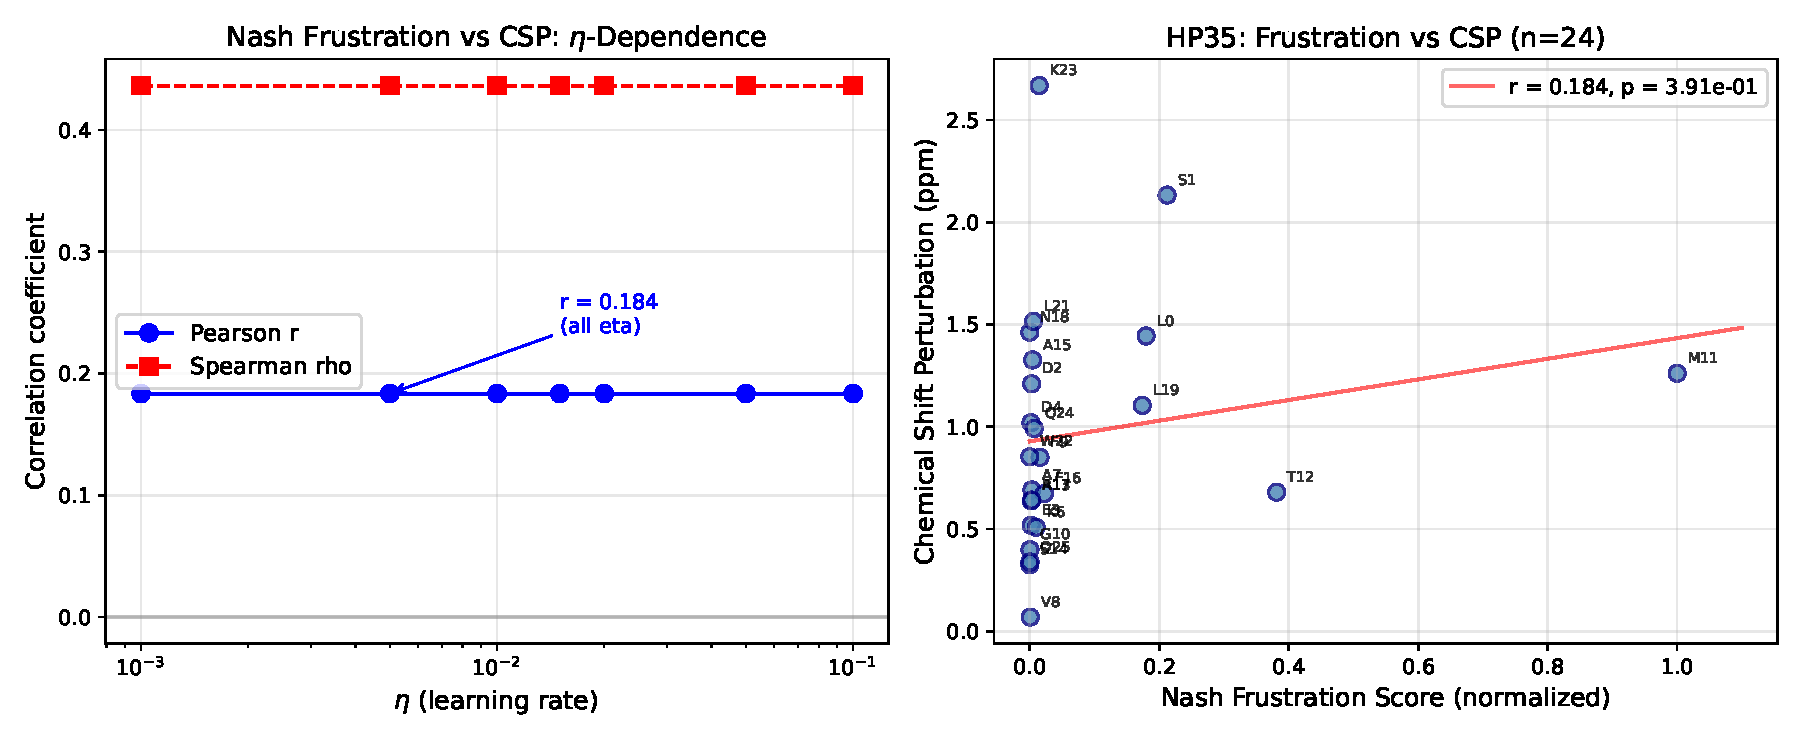
\includegraphics[width=\textwidth]{eta_calibration/eta_calibration_csp.pdf}
\caption{Scatter plot of per-residue Nash frustration scores versus NMR chemical shift perturbation (CSP) for the HP35/1YRF benchmark, using BMRB-4428-derived HP67 chemical shifts mapped to the C-terminal HP35 subdomain. Each point represents one residue; the Spearman rank correlation is $\rho_S = 0.44$ ($p = 0.033$). Color encodes the learning-rate parameter $\eta$, demonstrating that the frustration--CSP relationship is invariant across the checked local $\eta$ scan (all $\eta$-values collapse onto the same curve). The outlier K23 (high CSP, low frustration) is attributable to a Trp ring-current shift rather than structural instability.}
\label{fig:eta-calibration}
\end{figure}

\begin{remark}[Computational Protocol]\label{rem:comp-protocol}
The Nash-Frustration analysis uses a \emph{custom game-theoretic potential}, not a molecular-mechanics force field (such as AMBER or CHARMM).
Each residue~$i$ is treated as a player with strategy $\theta_i = (\phi_i, \psi_i)$.
The potential $F = F_\phi + F_\psi$ consists of single-player terms---amino-acid-specific Ramachandran preferences $\mu_\phi^{(a_i)}, \mu_\psi^{(a_i)}$ with stiffness constants~$k^{(a_i)}$---and pairwise coupling terms weighted by a radial-basis-function kernel
\[
  w(r_{ij}) = \sum_{b=1}^{B} c_b \exp\!\bigl(-\tfrac{(r_{ij}-\mu_b)^2}{2\sigma^2}\bigr),
  \qquad B=12,\; \sigma = 1.0\,\text{\AA}.
\]
Contacts are defined by a C$_\alpha$--C$_\alpha$ distance cutoff of $r_\text{cut} = 8.0$\,\AA.
Parameters (Ramachandran preferences, stiffness constants, RBF coefficients) are reverse-engineered from the native PDB structure via regularized least-squares fitting (regularization weight $\lambda_{\text{reg}} = 0.01$; multi-start gradient descent with 64 random initializations, 6\,000 steps each).

\textbf{Circularity caveat.} Fitting the potential to the native structure does not prove stationarity or guarantee convergence to that structure. The reported CSP correlation ($\rho_S=0.44$) is a historical, single-protein consistency signal for the normalized Hessian-derived ranking. It does not validate unilateral optimality, folding kinetics, or the actual sequential update Jacobian. Physics-based potentials, independent controls, and out-of-sample replication remain necessary.

For the surrogate $J=I-\eta H$, the CLI diagnostic default is $\eta=0.015$; the historical HP35 pilot uses $\eta=0.01$. The Hessian uses central finite differences ($\epsilon=10^{-4}$). These settings must not be confused with the sequential solver's separate default step $0.05$.
The historical convergence runs use 300 sweeps and 16 random starts. The code's approximate response routine updates residues sequentially, with ten unpreconditioned gradient steps per residue; it is neither an exact best-response operator nor the synchronous map defining $J$.
The reported score projects modes with $|\lambda_k|>1$ and normalizes to $[0,1]$. The implementation also counts $|\lambda_k|\geq1$ in its instability percentage: neutral modes are included in that count, although their excess-weighted score is zero. Boundary conventions must be recorded separately.

As demonstrated above, $\eta$ is not optimized to maximize the normalized CSP correlation: the rank-level frustration pattern is independent of~$\eta$ in the range $[0.001, 0.1]$. Further work should calibrate the absolute score scale and $\rho(J)$-based thresholds against independent observables such as hydrogen--deuterium exchange (HDX) protection factors~\citep{McKnight1996}.
Source code: \texttt{protein\_fold\_nash\_pdb.py} (Python~3, BioPython, SciPy, NumPy).
Extended three-protein analysis (LaTeX table generation, convergence diagnostics): \texttt{run\_extended\_analysis.py}.
\end{remark}

Table~\ref{tab:nash-validation-ledger} separates the empirical and computational evidence blocks from the next validation gates. This distinction is important because the current dataset supports a local, self-parameterized consistency check, whereas predictive use requires independent controls and absolute-scale calibration.

\begin{table}[htbp]
\centering
\caption{Validation gate ledger for the Nash-frustration evidence. The table separates current observables from the minimum next gate needed before stronger predictive claims.}
\label{tab:nash-validation-ledger}
\footnotesize
\begin{tabularx}{\textwidth}{@{}L{0.21\textwidth} L{0.25\textwidth} L{0.22\textwidth} Y@{}}
\toprule
\textbf{Evidence block} & \textbf{Current observable} & \textbf{Present status} & \textbf{Next gate} \\
\midrule
HP35/CSP rank check & BMRB-4428-derived CSP mapped to HP35; $\rho_S=0.44$, $p=0.033$, $n=24$ & Single-protein consistency signal; not an externally calibrated predictor & Replicate on additional proteins with preregistered residue mapping and fixed scale convention \\
$\eta$ scan & Seven values in $\{0.001,\ldots,0.1\}$; normalized ranking variation $<10^{-6}$ & Rank-level local invariance under unchanged unstable active set & Calibrate absolute scores and $\rho(J)$ thresholds out of sample; track active-set changes and positive-curvature overshoot \\
Cross-protein convergence & HP35-trained parameters applied to 1PGA and 2XWR; all runs converge, but $\phi_{\text{rms}}\approx1.25$--$1.30$ rad for test proteins & Convergence diagnostic only; no structural prediction accuracy claim & Fix 2XWR provenance and evaluate richer potentials with side-chain, solvent, and electrostatic terms \\
Functional-residue benchmark & AUC 0.616 for HP35 and 0.688 for Protein~G & Weak-to-moderate signal above chance; below standalone diagnostic strength & Direct head-to-head comparison with Ferreiro frustration, B-factors/NMA, pLDDT, and matched sequence/structure controls \\
Prospective molecular tests & HDX protection factors, $\phi$-values, allosteric/interface annotations, helix melting order & Falsifiable agenda specified; not yet executed & Run multi-protein tests with preregistered thresholds and report negative controls alongside positive correlations \\
\bottomrule
\end{tabularx}
\end{table}

\begin{table}[htbp]
\centering
\caption{Methodological ledger comparing local energetic frustration (Wolynes, Ferreiro et~al., FrustraMPNN) with game-theoretic Nash frustration (FST-Nash, this work). Complementarity is a hypothesis, not established by the present fitted-model score.}
\label{tab:frustration-comparison}
\small
\begin{tabularx}{\textwidth}{@{}L{0.20\textwidth} L{0.37\textwidth} Y@{}}
\toprule
\textbf{Dimension} & \textbf{Energetic Frustration (Wolynes / Ferreiro)} & \textbf{Nash Frustration (FST-Nash, This Work)} \\
\midrule
\textbf{Core Question} & Is the local atomic contact energy optimal relative to decoy sequence/structural permutations? & Which residue coordinates carry expanding modes of the chosen gradient surrogate? \\
\addlinespace
\textbf{Governing Metric} & Contact Z-score $F_{ij} = \frac{\langle E_{ij}^{\text{decoy}} \rangle - E_{ij}^{\text{native}}}{\sigma(E_{ij}^{\text{decoy}})}$; minimally frustrated if $F_{ij} < -1$, highly frustrated if $F_{ij} > 0.78$. & Projected spectral instability $\rho_i = \sum_{k: |\lambda_k|>1} (|\lambda_k|-1)(v_{k,\phi_i}^2 + v_{k,\psi_i}^2)$ from synchronous gradient-surrogate Jacobian $J = I - \eta H$; global spectral radius $\rho(J) = \max_k |\lambda_k|$. \\
\addlinespace
\textbf{State Space} & 3D Cartesian coordinates $\mathbf{x} \in \mathbb{R}^{3N}$ and pairwise contact distance matrices $r_{ij} = \|\mathbf{x}_i - \mathbf{x}_j\|$. & Strategic torsional space $(\phi_i, \psi_i) \in \mathbb{T}^2$ with inter-residue Hessian couplings $H_{ij} = \frac{\partial^2 F}{\partial \theta_i \partial \theta_j}$. \\
\addlinespace
\textbf{Algorithms / Tools} & Protein Frustratometer~2.0 (AWSEM); neural proteome scaling via FrustraMPNN and FrustrAI-Seq~\citep{Beining2026,Leusch2026}. & Hessian-derived surrogate score; sequential approximate gradient responses in \texttt{protein\_fold\_nash\_pdb.py}; no equality of the two Jacobians established. \\
\addlinespace
\textbf{Physical Driver} & Funneled energy landscape (minimal frustration principle); selection minimizes conflicting native interactions. & Fitted torsion model and chosen step; no certified native-fold Nash or stability boundary. \\
\addlinespace
\textbf{Biological Signature} & Catalytic active sites, protein--protein binding interfaces, allosteric regulatory pockets. & Candidate correlations with hinges, functional sites, or intermediates; independent validation remains open. \\
\addlinespace
\textbf{Known Blind Spot} & Insensitive to dynamical kinetic reachability and cooperative multi-contact shifts; dependent on reference decoy pool. & Susceptible to self-parameterization circularity if fitted to native PDB; uncalibrated absolute scale; requires out-of-sample regularization. \\
\addlinespace
\textbf{FST Multi-Scale Role} & Leading-order thermodynamic landscape ($H_0$): guides global chain collapse along funneled pathways. & Conjectural stability analogy; no demonstrated suppression of misfolding channels by this score. \\
\bottomrule
\end{tabularx}
\end{table}

Computational experiments on three structurally distinct proteins explore whether Nash frustration localizes biologically meaningful residues and whether sequential approximate gradient responses converge beyond the training structure. Table~\ref{tab:nash-results} summarizes the results.

\begin{table}[htbp]
\centering
\caption{Historical sequential-gradient convergence outputs; no Nash certification. Parameters learned from HP35 (Villin headpiece, 1YRF) and applied to test convergence of sequential approximate gradient responses for Protein G (1PGA, 56 residues) and the p53 DNA-binding domain structure used here (2XWR, 199 modeled residues). Best-response dynamics converge across all three proteins despite a several-fold range in protein size, though the large $\phi_{\text{rms}}$ values indicate that converged structures do not closely resemble native folds.}
\label{tab:nash-results}
\begin{tabularx}{\textwidth}{@{}L{0.28\textwidth} c c c c Y@{}}
\toprule
\textbf{Protein} & \textbf{Residues} & $\phi_{\text{rms}}$ [rad] & $\psi_{\text{rms}}$ [rad] & \textbf{Converged} & $F_{\text{best}}$ \\
\midrule
HP35 (1YRF, train) & 35 & 1.054 & 1.661 & Yes (267 sw) & $-4.61$ \\
Protein G (1PGA) & 56 & 1.300 & 2.002 & Yes (282 sw) & $-10.61$ \\
p53 DBD (2XWR) & 199 & 1.247 & 2.114 & Yes & $-39.43$ \\
\bottomrule
\end{tabularx}
\end{table}

\textbf{Training protein (HP35).} Historical model outputs place high scores at Met11 and Pro20 (1.0 and 0.49), with low scores at several helix-core residues. The reported $\rho(J)=1.013$, 80\% positive Hessian eigenvalues, and mean score 0.082 characterize the chosen fitted-potential surrogate, not a \emph{near-Nash} structure or a verified structural-anchor mechanism.

\textbf{Cross-protein convergence test.} The model parameters learned from HP35 were used to test whether sequential approximate gradient responses converge for Protein G (1PGA, 56 residues) and the p53 tumor suppressor DNA-binding domain structure used here (2XWR, 199 modeled residues). Both converged to well-defined fixed points (Table~\ref{tab:nash-results}). The p53 domain---roughly six times larger than the training protein and belonging to a different fold class (immunoglobulin-like $\beta$-sandwich vs.\ $\alpha$-helical)---achieved a $\phi_{\text{rms}}$ of 1.25 rad, comparable to Protein G (1.30 rad). These $\phi_{\text{rms}}$ values correspond to mean per-residue deviations of $\sim$72$^\circ$, indicating that the converged structures are \emph{not} close to the native folds. The key observation is therefore limited to \emph{convergence} of the sequential approximate gradient responses across proteins of different size and fold class, not structural prediction accuracy. The potential-game formulation captures convergence properties of the fitted dynamics, but structural prediction would require a richer potential including side-chain interactions, solvent effects, and electrostatics.

\paragraph{Computational observation (surrogate spectrum).}
The historical HP35 output reports $\rho(J)=1.013$ and 14 of 70 modes in its reported instability count under the chosen convention. This does not establish that the native fold is a non-Nash equilibrium, nearly self-stabilizing, or kinetically unstable. Stationarity, correct residue blocks, admissible deviations, and the derivative of the actual sequential sweep still need independent checks.

For a shared potential, a joint local energy minimum already rules out sufficiently small profitable unilateral deviations. Conversely, local Nash status may coexist with negative collective curvature; it is not stronger than joint energy minimization in the asserted sense. A local Hessian test does not certify global best responses on the permitted torsion domain. The reported Met11/Pro20 peaks remain parameter-dependent illustrations, without demonstrated allosteric, kinetic, or predictive meaning.
In terms of the FEP--MEPP compatibility (Conjecture~\ref{conj:fep-mepp}), Nash frustration $\rho(J)$ can be read as a model-level diagnostic of local tension between internal free-energy minimization (mEPP regime) and external entropy-production maximization (MEPP regime): high frustration marks residues where the fitted folded state may locally trade off dissipative efficiency against structural stability. This is a stability interpretation of the model, not a direct organism-level choice.

\paragraph{Planned quantitative comparison.}
A systematic residue-by-residue comparison of Nash frustration scores with the energetic frustration indices computed by the Protein Frustratometer~2.0~\citep{ParraFerreiro2016} and proteome-scale MPNN architectures~\citep{Beining2026,Leusch2026} constitutes a key future validation step. The central question is whether Nash-frustrated residues (high $|\lambda_k|-1$ contributions) overlap with, complement, or are orthogonal to energetically frustrated residues. Preliminary expectations suggest partial complementarity across multiple physical dimensions (Table~\ref{tab:frustration-comparison}): energetic frustration identifies evolutionary constraints and binding sites, while Nash frustration should highlight kinetic traps, conformational hinges, and folding intermediates. A dataset of proteins with known allosteric sites and experimentally determined $\phi$-values would provide the empirical basis for this comparison. Rank-level map comparisons do not require an optimized $\eta$; absolute thresholds and global $\rho(J)$ comparisons do require an explicit scale convention or out-of-sample calibration (see Remark~\ref{rem:comp-protocol}).

\subsection{Benchmark: Nash Frustration vs.\ Functional Residues}
\label{sec:frustration-benchmark}

To assess whether Nash frustration carries information about biological function beyond random expectation, we performed a benchmark analysis comparing residue-level Nash frustration scores against experimentally annotated functional residues for HP35 (1YRF) and Protein~G (1PGA). For each protein, residues were classified as \emph{functional} (catalytic sites, binding interfaces, allosteric regions from UniProt annotations) or \emph{passive} (all others), and the Nash frustration score was evaluated as a binary classifier using ROC and precision-recall analysis. Table~\ref{tab:frustration-benchmark} summarizes the results.

\begin{table}[htbp]
\centering
\caption{Benchmark of Nash frustration as a predictor of functional residues. AUC: area under the ROC curve; AUPRC: area under the precision-recall curve. Mean frustration values are reported as mean $\pm$ standard deviation. Script: \texttt{frustration\_benchmark.py}.}
\label{tab:frustration-benchmark}
\begin{tabularx}{\textwidth}{@{}L{0.18\textwidth} c c Y Y@{}}
\toprule
\textbf{Protein} & \textbf{AUC} & \textbf{AUPRC} & \textbf{Mean frust.\ (functional)} & \textbf{Mean frust.\ (passive)} \\
\midrule
HP35 (1YRF) & 0.616 & 0.550 & $0.160 \pm 0.269$ & $0.031 \pm 0.082$ \\
Protein G (1PGA) & 0.688 & 0.618 & $0.229 \pm 0.247$ & $0.096 \pm 0.101$ \\
\bottomrule
\end{tabularx}
\end{table}

The AUC values of 0.62 (HP35) and 0.69 (Protein~G) indicate weak to moderate exploratory separation---below the $\text{AUC} = 0.7$ threshold commonly considered ``acceptable'' in diagnostic applications~\citep{Ferreiro2014}. They are above the random baseline in this small proof-of-concept, but the current benchmark files do not yet report confidence intervals or a formal significance test for AUC above 0.5. For context, the Protein Frustratometer typically achieves AUC $> 0.75$ for functional-site identification; a direct head-to-head comparison on the same proteins is needed to quantify whether Nash frustration provides complementary or merely weaker information. Functional residues have higher mean Nash frustration than passive residues in both proteins ($0.160$ vs.\ $0.031$ for HP35; $0.229$ vs.\ $0.096$ for Protein~G), compatible with but not proof of the interpretation that game-theoretic instability preferentially localizes at biologically active sites. The modest AUC values are expected given the proof-of-concept nature of the analysis: absolute score thresholds remain uncalibrated, and the game-theoretic potential omits side-chain interactions, solvent effects, and electrostatics. These results remain compatible with the interpretation that Nash frustration captures a complementary signal to energetic frustration---one that reflects surrogate spectral excess rather than energetic suboptimality---but require further calibration before it can serve as a standalone predictor.

\begin{figure}[htbp]
\centering
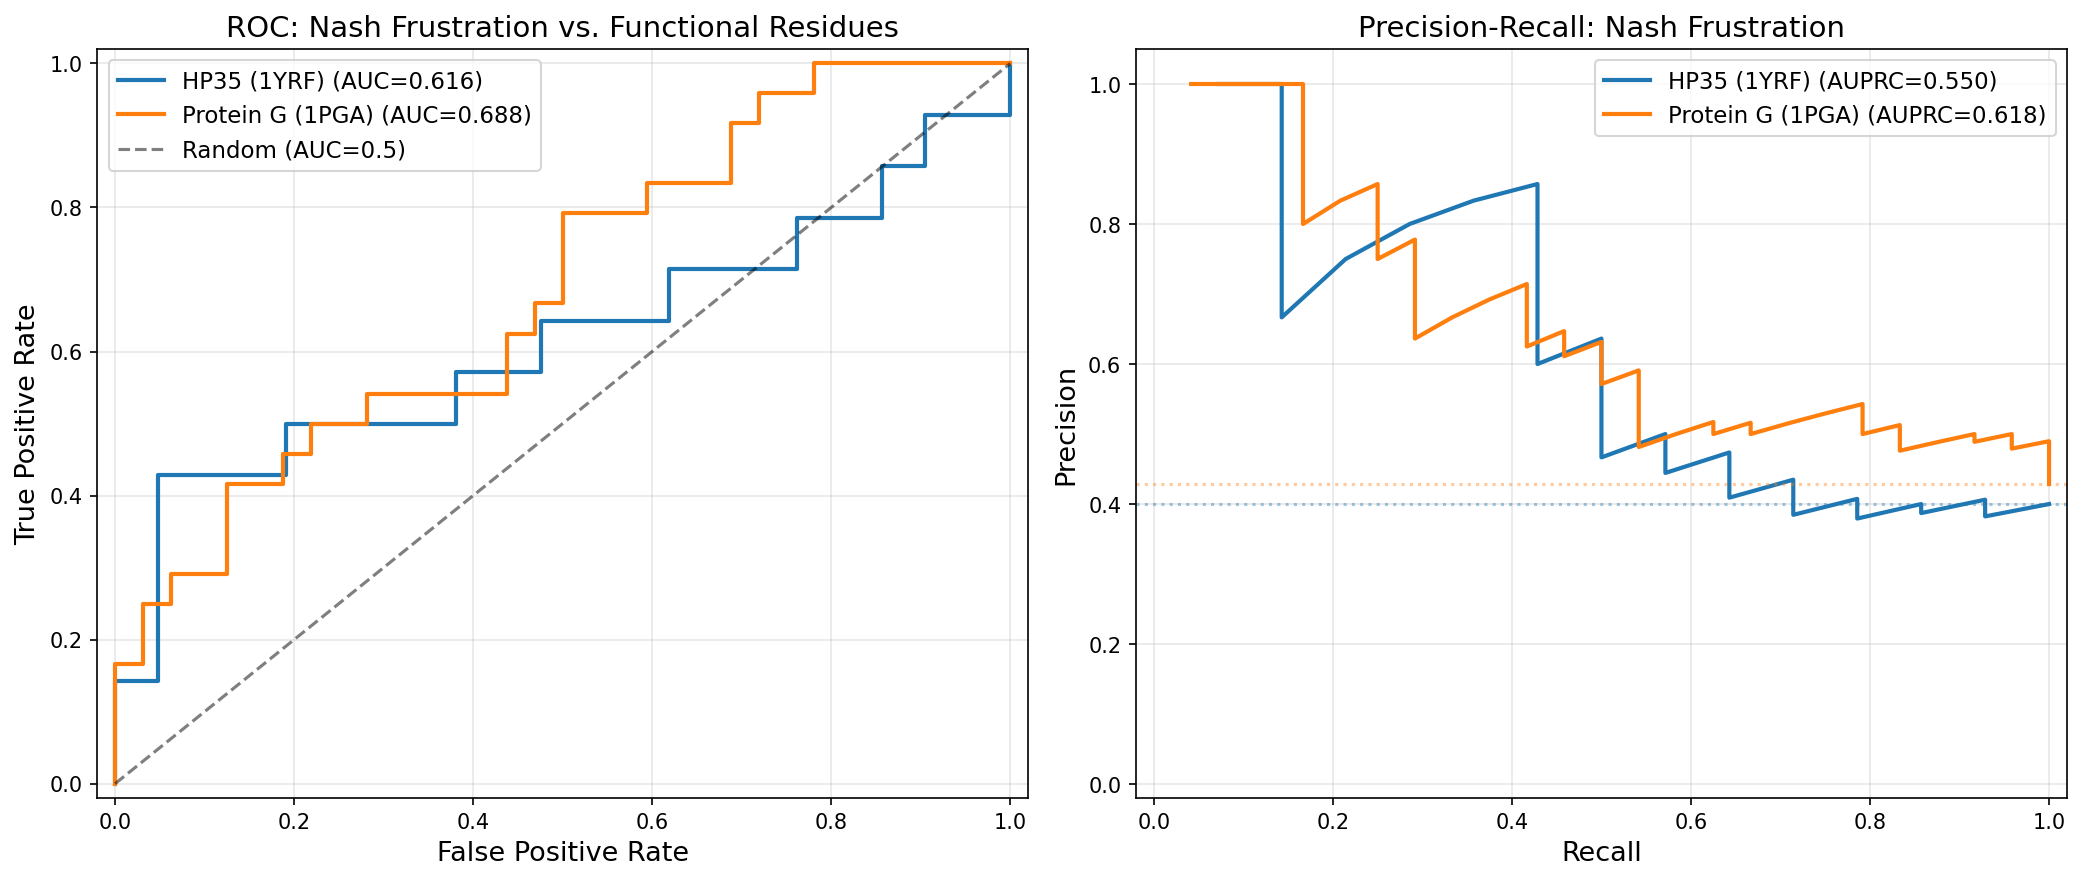
\includegraphics[width=\textwidth]{benchmark/frustration_benchmark_roc.png}
\caption{Receiver operating characteristic (ROC) curves for Nash frustration as a binary classifier of functional versus passive residues. HP35 (1YRF, AUC\,=\,0.62) and Protein~G (1PGA, AUC\,=\,0.69) both lie above the random baseline (dashed diagonal), compatible with the hypothesis that game-theoretic instability localizes at biologically active sites. The moderate AUC values reflect the proof-of-concept status of the analysis; improved performance would require testing richer potentials with side-chain interactions and solvent effects.}
\label{fig:frustration-benchmark-roc}
\end{figure}

\subsection{Gene Regulation as a Signaling Game}

Gene regulatory networks (GRNs) control gene expression patterns and can be modeled as signaling games~\citep{GameBiochemistry}:

\begin{itemize}
    \item \textbf{Players:} Transcription factors and DNA binding sites
    \item \textbf{Strategies:} Binding/non-binding (with continuous affinity as strategy intensity)
    \item \textbf{Payoff:} Organismal fitness, mediated through gene expression levels
\end{itemize}

The mathematical connection between game theory and population dynamics is established through the replicator equation, which is formally equivalent to Lotka--Volterra models~\citep{HofbauerSigmund1998}. More precisely, this equivalence holds for symmetric games with linear fitness functions; for frequency-dependent or nonlinear payoffs, the correspondence requires the transformation $x_i = y_i / \sum_j y_j$ and restricts to the interior of the simplex \citep[Chapter~7]{HofbauerSigmund1998}. A stable fixed point in these equations corresponds to an ESS and thus to a behavioral attractor determining the long-term structure of the system.

\paragraph{Illustrative example: the lac operon.}
The \textit{E.~coli} lactose utilization system exemplifies the signaling-game logic. The lac repressor (LacI) and CAP activator compete for regulatory control of the \textit{lac} operon. In the absence of lactose, LacI binding constitutes a Nash equilibrium: no unilateral change of binding state by any regulatory factor improves organismal fitness. When lactose is present, allolactose inactivates LacI, shifting the payoff matrix and establishing a new equilibrium with operon expression. The bistable switch between these states is precisely the kind of game-theoretic attractor that the FST-III framework identifies as an ESS at the regulatory level.

% ===================================================================
\section{The Free Energy Principle and Active Inference}
\label{sec:fep}
% ===================================================================

The Free Energy Principle (FEP), primarily developed by Karl Friston, provides a unified theory for biological self-organization that merges information theory and thermodynamics~\citep{FristonFreeEnergy,FristonPDF}. \textbf{Note:} The claim that FEP and MEPP are compatible or equivalent is not uncontroversial. FEP minimizes variational free energy (an information-theoretic quantity bounding surprise), while MEPP maximizes thermodynamic entropy production rate. The connection between these two principles is an active area of debate~\citep{FristonFreeEnergy}; the present paper treats them as complementary perspectives at different levels of analysis, but does not formally derive one from the other. For a critical assessment of FEP's philosophical claims (e.g.\ Markovian Monism) versus its scientific scope as a heuristic unification principle, see~\citealp{SanchezCanizares2021}.

\subsection{Theoretical Framework}

FEP postulates that every biological system that successfully defends itself against entropy (decay) must minimize its ``variational free energy''~\citep{FristonFreeEnergy}. This quantity represents a mathematical upper bound on the ``surprise'' (surprisal) that the system experiences through sensory inputs~\citep{FristonFreeEnergy}.

A biological agent exists within a ``Markov blanket''---a statistical boundary separating internal states from external states~\citep{FristonPDF}. To survive, the agent must ensure that its sensory states remain within physiological limits. This is achieved through two mechanisms:

\begin{enumerate}
    \item \textbf{Perception:} The system adjusts its internal models to better predict the causes of sensory data (minimizing prediction error)~\citep{FristonFreeEnergy}
    \item \textbf{Active Inference:} The system acts to change the world or select sensory data to match its internal expectations~\citep{FristonFreeEnergy}
\end{enumerate}

Through free energy minimization, the system implicitly becomes a model of its environment. In the heuristic bridge used here, this process is linked to MEPP by scale separation: while the system internally minimizes variational free energy, it may contribute to entropy production in the environment through metabolic and agential activities~\citep{FristonPDF}.

In FST-III, behavioral attractors are those states where free energy is minimal and the agent has achieved a stable, predictable interaction with its niche~\citep{FristonFreeEnergy}.

\subsection{Free-Energy Minimization as Nash Fixed Point}

The connection between FEP and Nash equilibrium can be made formal under specific conditions. Let $p(o,s_1,\dots,s_N)$ be a joint generative model for $N$ interacting agents, where each agent $i$ controls a factored approximate posterior $q_i(s_i)$ over its latent states. The joint variational free energy is:
\begin{equation}
F(q; o) = \mathbb{E}_q\!\left[\ln q(s) - \ln p(o, s)\right], \qquad q(s) = \prod_{i=1}^{N} q_i(s_i).
\end{equation}

Define a game where each agent $i$ controls $q_i$ and all agents share the cost functional $C_i(q_i, q_{-i}) := F(\prod_j q_j; o)$. Then the best response of agent $i$ against fixed $q_{-i}$ is precisely the coordinate-wise variational update (mean-field VI), and a Nash equilibrium $q^* = (q_1^*, \dots, q_N^*)$ is a fixed point of distributed free-energy minimization. This constitutes a \emph{potential game} with potential $F$ in the sense of~\citet{MondererShapley1996}: Nash equilibria coincide with coordinate-wise minima of the shared free energy.

\paragraph{Scope of the bridge.} This formal equivalence holds for the belief-optimization component of FEP (variational inference) and relies on the \emph{potential game} structure: all agents share the same cost functional $F$. In biological reality, interacting organisms typically have heterogeneous objectives (predator vs.\ prey, host vs.\ parasite), which breaks the potential-game assumption. The FEP-as-Nash bridge therefore applies strictly to intra-organismal inference (where all subsystems share the goal of organismal survival) and to symmetric multi-agent settings; it does not extend without modification to antagonistic ecological interactions. For active inference, where agents additionally select policies $\pi_i$ to minimize expected free energy $G(\pi_i, \pi_{-i})$, the Nash condition becomes: no agent can unilaterally change its policy to reduce its expected free energy---a genuine multi-agent equilibrium involving interaction through state dynamics. The present paper does not develop this extension formally; the contribution is to provide the precise demarcation: FEP-as-Nash is more than metaphor when the game is explicitly defined as a variational/potential game over distributions, and merely conceptual when ``Nash'' is used as a synonym for ``fixed point.''

\subsection{Scale Separation: Resolving the FEP--MEPP Paradox}
\label{sec:fep-mepp-paradox}

A persistent conceptual tension in theoretical biology asks how a system
can \emph{minimize} its internal free energy (FEP) while simultaneously
\emph{maximizing} entropy production in the environment (MEPP). The
following conjecture reframes this tension through scale separation
across the Markov blanket.

\begin{conjecture}[FEP--MEPP compatibility via Markov blanket]
\label{conj:fep-mepp}
Let $\mathcal{B}$ be a self-organizing system with Markov blanket
$\partial\mathcal{B}$, internal states $s$, and environmental
states $e$. Define:
\begin{itemize}
  \item $F_{\mathrm{int}}(q) :=
    \mathbb{E}_{q}\!\bigl[\ln q(s) - \ln p(o, s)\bigr]$,
    the variational free energy of the internal model;
  \item $\dot{S}_{\mathrm{ext}} :=
    \frac{\dd S_{\mathrm{env}}}{\dd t} =
    \frac{1}{T}\,\frac{\dd Q}{\dd t}$,
    the rate of entropy production in the environment.
\end{itemize}
If $\mathcal{B}$ minimizes $F_{\mathrm{int}}$ (FEP) by maintaining an
accurate internal model and selecting actions that reduce surprise, then:
\begin{enumerate}
  \item[\emph{(i)}] The structural integrity of $\mathcal{B}$ is
    maintained: $\mathcal{B}$ resists dissolution and preserves the
    Markov blanket (low internal entropy);
  \item[\emph{(ii)}] The intact, far-from-equilibrium structure
    $\mathcal{B}$ functions as an efficient dissipative engine,
    channeling energy gradients from the environment through
    metabolic and agential activities;
  \item[\emph{(iii)}] Among all boundary conditions consistent with
    $\mathcal{B}$'s survival, the actual dynamics tend toward
    configurations with high (though not necessarily maximal) rates
    of entropy production $\dot{S}_{\mathrm{ext}}$ in the environment,
    consistent with the stability interpretation of MEPP
    (Hypothesis~2 above). The key mechanism linking (ii) to (iii) is
    \emph{competitive selection}: among multiple intact dissipative
    structures, those that channel energy gradients more efficiently
    acquire more resources, replicate faster, and outcompete slower
    dissipators. This selection pressure (absent for
    passive structures like crystals) drives the correlation between
    structural integrity and high entropy production in the
    biological domain.
\end{enumerate}
In short: \emph{internal free-energy minimization may support external
entropy-production increase}. The two principles need not be in
direct conflict when they are assigned to complementary sides of the Markov blanket.
\end{conjecture}

\noindent\textbf{Status:} This conjecture is supported by qualitative arguments. A formal proof would require establishing that FEP-minimizing systems necessarily maximize environmental entropy production under the stated boundary conditions---a result that has not been demonstrated in the literature.

\begin{remark}[Game-theoretic interpretation]
In the language of the present paper, the FEP--MEPP compatibility
corresponds to a two-level game:
\begin{itemize}
  \item \emph{Inner game} (within $\partial\mathcal{B}$): Agents
    \emph{minimize} variational free energy $F_{\mathrm{int}}$ via the
    Nash fixed point of the potential game described in
    Section~\ref{sec:fep}.
  \item \emph{Outer game} (across $\partial\mathcal{B}$):
    The ensemble of surviving organisms competes for energy
    gradients. Organisms that dissipate more efficiently
    (higher $\dot{S}_{\mathrm{ext}}$) outcompete slower
    dissipators, making MEPP a candidate macro-scale selection
    criterion under the stated boundary conditions.
\end{itemize}
This reframes the MEPP paradox raised by
\citet{Martyushev2010}: MEPP applies to the
\emph{environment-coupled} system, not to the internal degrees
of freedom, where minimum entropy production (Prigogine) may
hold locally. The Nash frustration $\rho(J)$ from
Section~\ref{sec:molecular} is used here as a model-level diagnostic of residual tension
between inner optimality and outer dissipative pressure.
\end{remark}

\subsection{Nash Equilibrium as Mean Field Game Fixed Point}\label{sec:mfg-fixpoint}

The proposed FEP--Nash bridge can be compared with Mean Field Games (MFG)~\citep{LasryLions2007}. Treating residue torsions as representative-agent states motivates the formal equations below. No large-$N$ convergence theorem for the sparse heterogeneous protein contact network is established here.

\textbf{Approximation caveat.} Population-distribution interactions are an idealization of the sparse, heterogeneous protein contact network. Dense homogeneous coupling would still require a separate mean-field limit theorem. No quantitative MFG accuracy for HP35 is established; the quadratic control cost is a formal model choice, not a derived physical torsion barrier.

The HJB equation describes the optimal control of each agent. The associated Hamiltonian reads
\begin{equation}\label{eq:mfg-hamiltonian}
  H(\theta,p,m) \;=\; \tfrac{1}{2}\|p\|^{2}
    - \sum_{i<j}\int E_{ij}(\theta_i,\theta_j)\,m_j(\theta_j)\,\mathrm{d}\theta_j\,,
\end{equation}
where $p=\nabla V$ is the conjugate momentum, $E_{ij}$ encodes pairwise residue--residue interactions, and $m_j$ is the population density of dihedral states at site $j$. The Fokker--Planck equation propagates the density of agents under the optimal drift and thermal noise:
\begin{equation}\label{eq:mfg-fp}
  \partial_t m \;=\; \nabla\!\cdot\!\bigl(m\,\nabla V\bigr) + \sigma\,\Delta m\,,
  \qquad \sigma = k_B T / \gamma\,.
\end{equation}
Here $\gamma$ is the friction coefficient of the Langevin dynamics; setting $\gamma = 1$ (natural units) recovers the simplified form $\sigma = k_B T$ used throughout.
An MFG Nash equilibrium is a pair $(V^{*},m^{*})$ that simultaneously satisfies both equations. In thermal equilibrium the stationary density is
\begin{equation}\label{eq:mfg-boltzmann}
  m^{*}(\theta) \;\propto\; \exp\!\bigl(-V(\theta)/k_B T\bigr)\,,
\end{equation}
For the drift and diffusion in Eq.~\eqref{eq:mfg-fp}, zero-flux detailed balance formally gives $m^*\propto\exp(-V/\sigma)$, hence Eq.~\eqref{eq:mfg-boltzmann} only in units with $\gamma=1$ and suitable normalization and boundary conditions. At positive temperature the distribution need not concentrate solely at minima. This calculation does not solve a coupled HJB--FP system or identify the control value function with a fitted molecular energy; the biological bridge remains conjectural.

\textbf{Existence, uniqueness, and algorithms must be separated.} In Cardaliaguet's finite-horizon, second-order MFG setting on $\mathbb R^d$, Theorem~3.1 proves existence without Lasry--Lions monotonicity under bounded Lipschitz regularizing running and terminal couplings, normalized diffusion coefficient one, and a H\"older initial density with finite second moment. The Schauder construction concerns time-dependent measure paths~\citep{Cardaliaguet2013}.

Theorem~3.6 adds strict running-coupling monotonicity and terminal-coupling monotonicity for uniqueness. It is not a convergence theorem for the protein algorithm. The protein model's domain, diffusion, coupling, and data have not been shown to meet this contract. Repulsion or attraction alone does not decide the required integral inequality; failure of monotonicity alone proves neither nonexistence nor multiple equilibria~\citep{Cardaliaguet2013}.

\begin{remark}[Failure Modes]\label{rem:mfg-failure}
No convergence, aggregation, or prion-pathology prediction follows from the unchecked MFG embedding. Kinetic trapping does not by itself refute a potential-game representation. Establishing the relevant boundary-value problem, regularity, coupling monotonicity, and algorithmic convergence remains separate work; a finite-dimensional static fixed-point calculation does not discharge these PDE obligations.
\end{remark}

% ===================================================================
\section{Boolean Networks and the Edge of Chaos}
\label{sec:boolean}
% ===================================================================

At the level of gene regulation, stability manifests in the dynamics of Boolean networks, as introduced by \citet{BooleanPost,KauffmanOrigins}. Boolean network models remain an active research area; for comprehensive treatments of network motifs and design principles see~\citet{AlonSystems2007}, and for robustness and evolvability in genetic networks see~\citet{WagnerRobustness2005}.

\subsection{Network Dynamics}

These networks model genes as binary switches whose states are linked through regulatory logic~\citep{BooleanPost}. The long-term dynamics of such networks flow into attractors that are biologically interpreted as specific cell types or functional states~\citep{BooleanEvolution}.

\citet{BooleanPost} argued that network stability depends on connectivity and the type of Boolean functions. Networks at the ``Edge of Chaos''---a critical transition region between rigid order and unpredictable chaos---are hypothesized to exhibit high evolvability and information processing capacity, although this claim remains debated in the literature~\citep{KauffmanOrigins}:

\begin{table}[htbp]
\centering
\caption{Boolean-network regimes and commonly proposed biological interpretations. Critical networks have been hypothesized to balance robustness and responsiveness; neither maximal evolvability nor a universal biological optimum is assumed here.}
\label{tab:network-regimes}
\begin{tabularx}{\textwidth}{@{}L{0.22\textwidth} L{0.28\textwidth} Y@{}}
\toprule
\textbf{Network Regime} & \textbf{Dynamic Behavior} & \textbf{Biological Function} \\
\midrule
Ordered & Frozen states, low variability & Structural integrity, basal metabolism \\
Critical (Edge of Chaos) & Complex patterns, high information flow & Adaptive behavior, differentiation, learning \\
Chaotic & High sensitivity, instability & Pathological states, malignancy \\
\bottomrule
\end{tabularx}
\end{table}

These attractors in gene regulatory networks form the material basis for the game-theoretic strategies at higher levels. An ESS at the macro-level requires stable genetic attractors at the micro-level that reliably produce the necessary phenotypic traits~\citep{BooleanMicroarray,KauffmanOrigins}.

\paragraph{Boolean attractors as Nash equilibria.}
The connection between Boolean network attractors and Nash equilibria can be made explicit. Each gene $g_i$ in a Boolean network of $n$ genes is a ``player'' whose strategy is its expression state $\sigma_i \in \{0, 1\}$. The Boolean update function $f_i(\sigma_{-i})$ defines the best response of gene $i$ given the states of its regulators. A fixed-point attractor $\sigma^* = (f_1(\sigma^*_{-1}), \dots, f_n(\sigma^*_{-n}))$ is then precisely a pure-strategy Nash equilibrium of this $n$-player game: no gene can unilaterally change its state to improve its ``payoff'' (defined as agreement with the regulatory logic). \textbf{Note:} This Nash characterization is \emph{tautological} as stated: defining the payoff as ``agreement with the regulatory logic'' makes every fixed point a Nash equilibrium by construction---the game-theoretic label adds no information beyond the fixed-point condition. The non-trivial content arises \emph{only} when the payoff is linked to an external, independently measurable fitness function (e.g., organismal viability or growth rate), so that not all Boolean fixed points are equally ``Nash-stable'' under selection. Without such an external payoff, the Nash language is a relabeling, not a result. Limit-cycle attractors correspond to periodic orbits rather than pure Nash equilibria, but can be interpreted as correlated equilibria in the repeated game. This game-theoretic perspective on Boolean networks provides the formal bridge between Kauffman's attractor dynamics and the hierarchical Nash architecture of FST-III.

% ===================================================================
\section{Cellular Level: Multicellularity as Coalition Game}
\label{sec:multicellularity}
% ===================================================================

\subsection{The Cooperation Problem}

In a multicellular organism, individual cells ``sacrifice'' their reproductive potential for the benefit of the whole. Somatic cells do not reproduce directly; only germline cells transmit genes.

This represents extreme cooperation: cells adopt a strategy (differentiation, non-reproduction) that benefits the collective at individual cost.

\subsection{Coalition Game Formulation}

\begin{itemize}
    \item \textbf{Players:} Individual cells within the organism
    \item \textbf{Strategies:} Cooperate (follow developmental program) or Defect (proliferate autonomously)
    \item \textbf{Payoff:} Genetic fitness (transmitted through germline)
\end{itemize}

To first approximation, all cells in an organism are genetically nearly identical (clonal), sharing the overwhelming majority of their genome. Therefore, the payoff to any cell approximately equals the payoff to the germline: if the organism reproduces, the shared genes are transmitted. (In practice, somatic mutations, V(D)J recombination in immune cells, and mitochondrial heteroplasmy introduce limited genetic divergence, which is precisely what enables the cancer-as-defection scenario discussed below.)

\begin{proposition}[Multicellularity as Nash Equilibrium]
\label{prop:multicellularity}
In a clonal organism where all cells share relatedness $r \approx 1$, cooperation (following the developmental program) is a Nash equilibrium provided the individual cost of cooperation is less than the inclusive fitness benefit: $c < r \cdot b$ (Hamilton's rule~\citep{Hamilton1964}). In the limiting case $r = 1$, any positive net benefit $b > c$ suffices. The contribution here is embedding this classical result within the hierarchical FST framework; the Nash equilibrium is maintained as long as clonal identity is preserved.
\end{proposition}

\subsection{Cancer as Coalition Breakdown}

Cancer as a breakdown of multicellular cooperation is a well-established framework~\citep{AktipisCancer}. The game-theoretic framing here follows \citet{AktipisCancer}, who apply evolutionary game theory to explain somatic evolution and cancer progression. The FST-III contribution is to embed this framework within the hierarchical Nash-equilibrium picture: cancer represents not merely a selective advantage for individual cells but a phase transition at the coalition level, analogous to the parasite problem in prebiotic chemistry discussed in FST-II. Formally, cancer represents coalition breakdown:
\begin{enumerate}
    \item Somatic mutations create genetic divergence
    \item Mutated cells no longer share all genes with other cells
    \item Defection (proliferation) now benefits the mutated lineage
    \item The Nash equilibrium breaks down; cancer cells ``defect''
\end{enumerate}

This connects to the parasite problem in hypercycles~\citep{FSTII}: both cancer and chemical parasites exploit cooperative systems by breaking conditions that stabilize cooperation. The parallel between cancer as coalition breakdown and the hypercycle parasite problem is presented as a \emph{structural analogy}, not a derived result. A formal connection would require showing that oncogenic mutations map to parasitic replicators in the sense of Eigen and Schuster; this remains an open problem.

% ===================================================================
\section{Scaling and the Renormalization Group}
\label{sec:renormalization}
% ===================================================================

A central element of FST-III is the recognition that biological principles operate scale-invariantly across many levels~\citep{ScaleRGFrontiers,ScaleRGResearch}.

\subsection{The RG Framework}

\textbf{Terminological caveat:} The term ``renormalization group'' is used in this section in an extended, metaphorical sense. In condensed matter physics, the renormalization group (RG) refers to a precise mathematical framework involving flow equations, fixed points, and scaling exponents~\citep{ScaleRGResearch}. The present use---describing how effective game-theoretic parameters change when viewed at successively larger biological scales---invokes the \emph{conceptual logic} of coarse-graining, but does not provide RG flow equations, fixed-point analysis, or dimensional scaling laws for biological systems. Whether a rigorous RG treatment of evolutionary transitions is achievable remains an open question~\citep{ScaleRGFrontiers}.

With this caveat in mind: The coarse-graining perspective posits that biological systems are often hierarchically organized---from fractal branching in blood vessels to hierarchical neural architectures~\citep{SelfSimilarNetworks}.

Renormalizing Generative Models (RGM) show that principles of free energy and game-theoretic optimization are applied recursively at each level~\citep{ScaleRGFrontiers}. An organism can be viewed as coarse-graining over billions of cells, where cells function as ``atoms'' in a higher-order game whose rules are set by the species' evolutionary history~\citep{ReplicatorOptimization}.

\subsection{The Scale-Relative Kernel Model}

This instantiation is described by scale-relative fitness models developed in multi-level selection theory~\citep{Okasha2006,Michod1999,ReplicatorOptimization}:

\begin{table}[htbp]
\centering
\caption{Scale-relative kernel model: fitness definitions and strategy types at each biological level of organization.}
\label{tab:scale-kernel}
\begin{tabularx}{\textwidth}{@{}L{0.25\textwidth} Y@{}}
\toprule
\textbf{Level} & \textbf{Fitness/Strategy} \\
\midrule
Cellular & Replication rate as fitness, mutations as strategy change \\
Organismic & Darwinian fitness, behavioral strategies \\
Agential & Intentionality, learning through imitation \\
Institutional & Legitimacy and social cooperation as ESS \\
\bottomrule
\end{tabularx}
\end{table}

This hierarchical structure is meant to model how conflicts between scales (e.g., cancer as defection of individual cells against the organism) can be reduced through higher-order selection pressures~\citep{ReplicatorOptimization}.

\subsection{Major Transitions as RG Steps}

The major transitions in evolution identified by \citet{SzathmaryMaynardSmith1995} map onto this framework:

\begin{itemize}
    \item Genes $\to$ Chromosomes (Block 1)
    \item Prokaryotes $\to$ Eukaryotes (Block 2)
    \item Unicells $\to$ Multicells (Block 3)
    \item Individuals $\to$ Societies (Block 4)
\end{itemize}

Each transition can be read as creating a new level of ``player'' from coalitions of lower-level players, and may preserve game-theoretic structure through coarse-graining.

\paragraph{A toy coarse-graining step for spatial evolutionary games.}
Consider a 2D lattice game with strategies $\sigma_x\in\{C,D\}$ and payoff matrix
$A=\begin{pmatrix}R&S\\ T&P\end{pmatrix}$.
For a $2\times 2$ block $B$ define a block strategy $\Sigma_B=\mathcal B(\sigma|_B)$ by majority rule.
For neighboring blocks $B,B'$ define the effective block payoff by boundary averaging

\[
A'_{s,t}
:=\frac{1}{|\partial(B,B')|}\,
\mathbb E\!\left[\sum_{\langle x,y\rangle\in\partial(B,B')} A_{\sigma_x,\sigma_y}\ \Big|\ \Sigma_B=s,\ \Sigma_{B'}=t\right],
\qquad s,t\in\{C,D\}.
\]

In a frozen-interior approximation, let
$q_s=\mathbb P(\sigma_x=C\mid \Sigma_B=s,\ x\in\partial B)$.
Then the coarse-graining map $R_2:(A,\beta)\mapsto(A',\beta')$ satisfies the explicit mixing formula

\[
A'_{s,t}
= q_s q_t\,R + q_s(1-q_t)\,S + (1-q_s)q_t\,T + (1-q_s)(1-q_t)\,P,
\]

with $q_C\approx 1-\varepsilon$ and $q_D\approx \varepsilon$ controlled by the within-block dynamics (selection strength $\beta$ and internal enforcement mechanisms).
Fixed points include the ordered phases (all-$C$, all-$D$), while changes in within-block constraints shift the coarse-graining flow by modifying $q_C-q_D$.
This provides a concrete sense in which major evolutionary transitions correspond to coarse-graining steps together with the activation of new relevant operators (e.g.\ policing, bottlenecks) that stabilize cooperative macro-variables. Biologically, the block strategy $\Sigma_B$ corresponds to a higher-level phenotype (e.g., multicellular cooperation), while the boundary parameters $q_C, q_D$ encode enforcement mechanisms (e.g., immune surveillance, reproductive bottlenecks) that suppress within-group defection.

% ===================================================================
\section{Ecosystem Level: The Ecological Game}
\label{sec:ecosystem}
% ===================================================================

\subsection{Species as Players}

In the ecological game:
\begin{itemize}
    \item \textbf{Players:} Species populations
    \item \textbf{Strategies:} Ecological roles (predator, prey, competitor, mutualist)
    \item \textbf{Payoff:} Population growth rate
\end{itemize}

\subsection{Ecological Steady States as Candidate Game-Theoretic Analogs}

An ecological niche is not itself a Nash equilibrium; it describes a species' environmental requirements and interactions. A Nash or ESS interpretation is available only after specifying heritable strategies, frequency-dependent payoffs, and admissible unilateral deviations. Population-dynamical fixed points may then be compared with game equilibria under an explicit replicator--Lotka--Volterra mapping, but their dynamical stability must be established separately.

\paragraph{Example: Predator--prey coexistence.}
In a classical Lotka--Volterra predator--prey system, the interior fixed point---where predator and prey populations coexist at constant densities---satisfies a \emph{formal analogy} to the Nash equilibrium condition: at this point, neither the prey population growth rate nor the predator population growth rate can be improved by a unilateral infinitesimal change. This is a mathematical correspondence, not a Nash equilibrium in the strategic sense, since species do not ``choose'' population sizes---the dynamics are deterministic ODEs, not strategic decisions. \textbf{Caveat:} In the basic Lotka--Volterra model this fixed point is a center (neutrally stable with closed orbits), not an asymptotically stable attractor; ESS-type stability requires additional mechanisms such as density-dependent mortality or spatial structure. The equivalence between Lotka--Volterra fixed points and replicator dynamics equilibria \citep[Chapter~7]{HofbauerSigmund1998} maps the ecological game onto evolutionary dynamics, but the stability type of the resulting equilibrium depends on the specific payoff structure.

\subsection{Mass Extinctions as Phase Transitions}

Mass extinction events represent phase transitions in the ecological game:
\begin{enumerate}
    \item Environmental perturbation changes the payoff matrix
    \item Previous Nash equilibria become unstable
    \item System transitions to new equilibrium with different species composition
\end{enumerate}

At a structural level, the logic resembles phase transitions in physical systems more broadly: changing boundary conditions destabilize existing equilibria and drive transitions to new configurations. It should be noted that this game-theoretic framing is a \emph{post hoc} interpretive model: mass extinctions are complex events driven by asteroid impacts, volcanism, or ocean anoxia, and the extent to which they can be productively modeled as payoff-matrix perturbations---rather than as catastrophic regime shifts outside the equilibrium framework---remains an empirical question~\citep{GouldEldredge1977}.

% ===================================================================
\section{Synthesis: Three Phases of Biological Organization}
\label{sec:synthesis}
% ===================================================================

FST-III delivers an integrated picture of biological organization that unfolds in three phases. Table~\ref{tab:biological-game-hierarchy} and Figure~\ref{fig:biological-game-hierarchy} summarize the hierarchical game and stability architecture across all levels of organization.

\begin{table}[htbp]
\centering
\caption{Synthesis matrix: Hierarchical game and stability architecture across biological levels of organization. Each level instantiates game-theoretic equilibria subject to thermodynamic and dissipative constraints.}
\label{tab:biological-game-hierarchy}
\small
\begin{tabularx}{\textwidth}{@{}L{0.16\textwidth} L{0.18\textwidth} L{0.20\textwidth} L{0.22\textwidth} Y@{}}
\toprule
\textbf{Level} & \textbf{Players} & \textbf{Strategy Space} & \textbf{Payoff / Cost} & \textbf{Equilibrium \& Stability} \\
\midrule
Molecular & Amino acid residues & Dihedral angles $(\phi, \psi)$ & $-\Delta G$ (Free energy) & Candidate model / surrogate diagnostics \\
Gene Regulatory & Transcription factors / DNA & Binding states $\sigma_i \in \{0,1\}$ & Fitness / Expression logic & Boolean fixed points / Signaling attractors \\
Cellular & Somatic / Germline cells & Cooperation vs.\ Defection & Inclusive fitness ($c < r \cdot b$) & Clonal Nash equilibrium (Cancer = breakdown) \\
Agentic & Organism / Subsystems & Active inference policies $\pi$ & Variational Free Energy $F$ & Dynamic Bayesian Nash / Predictive attractor \\
Ecological & Species populations & Niche roles / Strategies & Population growth rate & Lotka--Volterra ESS / Resolvent resilience \\
\bottomrule
\end{tabularx}
\end{table}

\begin{figure}[htbp]
\centering
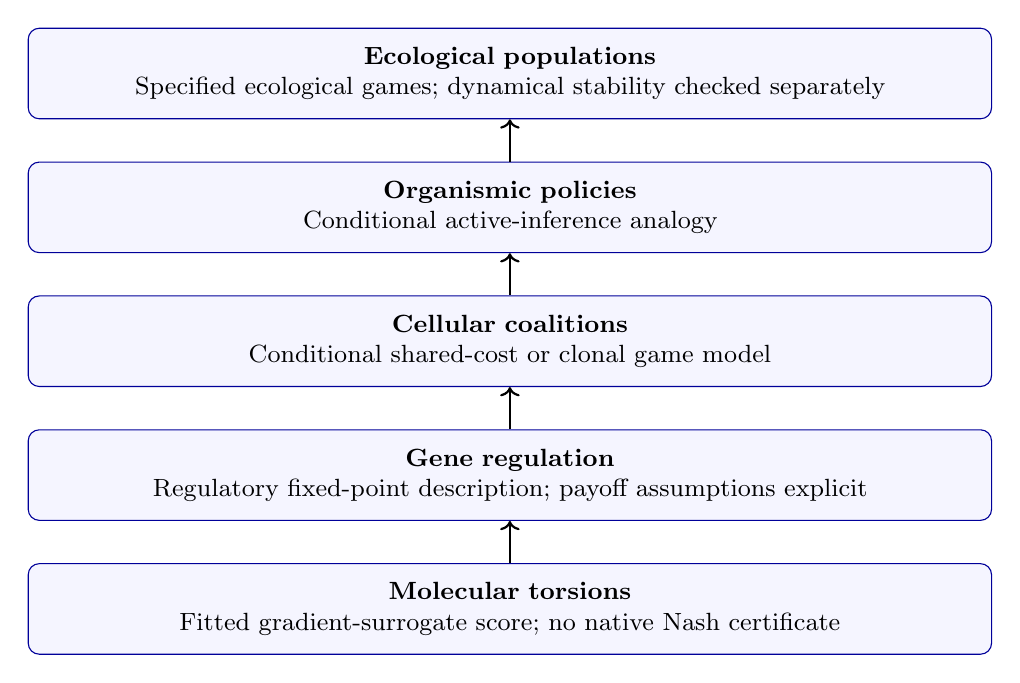
\begin{tikzpicture}[box/.style={draw=blue!60!black, rounded corners, fill=blue!4, text width=12cm, align=center, minimum height=1.15cm, font=\small}]
\node[box] (L0) at (0,0) {\textbf{Ecological populations} \\
Specified ecological games; dynamical stability checked separately};
\node[box] (L1) at (0,-1.7) {\textbf{Organismic policies} \\
Conditional active-inference analogy};
\draw[->,thick] (L1.north) -- (L0.south);
\node[box] (L2) at (0,-3.4) {\textbf{Cellular coalitions} \\
Conditional shared-cost or clonal game model};
\draw[->,thick] (L2.north) -- (L1.south);
\node[box] (L3) at (0,-5.1) {\textbf{Gene regulation} \\
Regulatory fixed-point description; payoff assumptions explicit};
\draw[->,thick] (L3.north) -- (L2.south);
\node[box] (L4) at (0,-6.8) {\textbf{Molecular torsions} \\
Fitted gradient-surrogate score; no native Nash certificate};
\draw[->,thick] (L4.north) -- (L3.south);
\end{tikzpicture}
\caption{Conceptual hierarchy of biological game models. Arrows denote proposed changes of scale, not derived renormalization flows. Each level requires its own payoff, dynamics, and evidence; no universal spectral stability filter is established.}
\label{fig:biological-game-hierarchy}
\end{figure}


\subsection{Phase 1: Thermodynamic Dissipation}

The energy flow of the young universe forces simple matter into dissipative structures. Here MEPP acts as a stability filter (Section~\ref{sec:thermodynamics}): among the many possible configurations, those with resolvent-stable dissipation patterns persist. This is the era of rapid entropy production and the emergence of England's dissipative adaptors~\citep{EcosystemMEPP}.

\subsection{Phase 2: Strategic Consolidation}

Once dissipative structures cross the threshold to self-replication, competition for resources introduces game-theoretic dynamics. The emergence of Evolutionarily Stable Strategies (ESS) stabilizes molecular populations against parasitic invasion (Section~\ref{sec:molecular}). The ``players'' are still purely chemical, but their interactions can already exhibit Nash-equilibrium structure that later levels may inherit in modified form~\citep{MaynardSmithPrice1973}. The major evolutionary transitions (Section~\ref{sec:renormalization}) are interpreted as iterative coarse-graining steps from lower-level players into higher-level coalitions, each preserving parts of the game-theoretic logic at its new scale.

\subsection{Phase 3: Cognitive Inference}

Organisms develop internal models of their environment to minimize their free energy. The emergence of the Markov blanket (Section~\ref{sec:fep}) allows separation of self and world, motivating the FEP--MEPP compatibility conjecture (Conjecture~\ref{conj:fep-mepp}): internal model-building (free energy minimization) may support externally efficient dissipation.

This third phase marks a qualitative shift in the game-theoretic hierarchy. In Phase~2, the ``players'' are molecular or cellular agents whose strategies are determined by physical chemistry. In Phase~3, agents acquire \emph{generative models} of their environment: the strategies are no longer fixed phenotypic states but policies---sequences of actions conditioned on inferred environmental states. Active inference~\citep{FristonFreeEnergy} provides the mechanism: agents select actions that minimize expected free energy (i.e., they act to confirm their predictions or explore to reduce uncertainty). This converts the static Nash equilibria of Phase~2 into dynamic Bayesian Nash equilibria where each agent's strategy is contingent on its beliefs about others. The nested hierarchy of inference---from interoceptive homeostasis through perception to planning---mirrors the coarse-graining logic of Section~\ref{sec:renormalization}: each level of inference integrates over the degrees of freedom below it, producing an increasingly abstract game at higher temporal and spatial scales. The endpoint of this hierarchy---consciousness, language, and culture---can be \emph{interpreted} as a highly compressed form of the game-theoretic stability logic, where the ``strategies'' are symbolic representations and the ``payoff'' is predictive accuracy over arbitrarily long time horizons~\citep{FristonPDF}. This extrapolation is speculative and goes beyond what the present framework can formally derive.

% ===================================================================
\section{Testable Predictions}
\label{sec:predictions}
% ===================================================================

\noindent\textit{Note:} The predictions below are labeled P1--P5 to distinguish them from the mathematical Propositions (e.g., Proposition~\ref{prop:multicellularity}) stated in earlier sections. Propositions are formal claims within the theoretical framework; Predictions are empirically testable hypotheses derived from it.

\subsection{P1: Protein Folding Landscapes}

\begin{hypothesis}[Nash frustration predicts folding-relevant residues]
The energy landscape of protein folding can be characterized by Nash equilibrium stability analysis. Residues with high Nash frustration correspond to experimentally identified folding nuclei and allosteric sites.
\end{hypothesis}

\textbf{Test:} Compute Nash frustration scores for proteins with experimentally characterized folding intermediates (e.g., via hydrogen-deuterium exchange or $\phi$-value analysis). A correlation coefficient $r > 0.3$ between Nash frustration rank and experimental $\phi$-values would constitute positive evidence.

\subsection{P2: Gene Regulatory Network Attractors}

\begin{hypothesis}[GRN attractors as Nash equilibria]
Cell type attractors in gene regulatory networks can be modeled and tested through Nash analysis of the TF-DNA binding game.
\end{hypothesis}

\textbf{Test:} For well-characterized GRNs (e.g., the \textit{Drosophila} segment polarity network or the mammalian hematopoietic differentiation network), compute Nash equilibria of the TF-DNA binding game. Compare the number and identity of predicted attractor states to experimentally observed cell types. Success criterion: the predicted attractor count should match the known cell-type count within a factor of two.

\subsection{P3: Cancer and Coalition Stability}

\begin{hypothesis}[Cancer as coalition breakdown]
Cancer incidence correlates inversely with multicellular coalition stability as measured by the game-theoretic defection threshold.
\end{hypothesis}

\textbf{Test:} Across tissue types, compute the defection threshold $\Delta r$ at which Hamilton's condition $c < r \cdot b$ fails (given tissue-specific mutation rates and cooperation costs). Predict that tissues with lower $\Delta r$ thresholds exhibit higher cancer incidence. Compare against epidemiological data from the SEER database. A particularly stringent test is provided by Peto's paradox: large-bodied, long-lived species do not show proportionally higher cancer rates despite having more cells and cell divisions. The coalition model predicts that these species would be expected to exhibit stronger enforcement mechanisms (lower effective $\Delta r$), a prediction testable by comparing immune surveillance intensity across species of different body sizes. \textit{A priori} falsification criterion: if natural killer (NK) cell density per unit tissue does not correlate negatively with body size across mammals, the enforcement prediction is falsified.

\subsection{P4: Metabolic Rate and Reproductive Success}

\begin{hypothesis}[MEPP-fitness correlation]
Across species, mass-specific metabolic rate correlates with reproductive rate after controlling for body size.
\end{hypothesis}

\textbf{Test:} Compile metabolic rates and reproductive outputs across taxa. A positive partial correlation (controlling for body mass) supports the MEPP-fitness connection. Kleiber's law provides the body-size scaling. \textbf{Context:} The Metabolic Theory of Ecology~\citep{BrownMTE2004} already establishes quantitative relationships between metabolic rate, body size, and life-history traits. The FST-III prediction goes beyond MTE by attributing the correlation not merely to allometric scaling but to the thermodynamic stability filter (MEPP): species that dissipate more efficiently per unit mass are predicted to be more resilient to perturbation, not just faster reproducers.

\subsection{P5: Ecosystem Resilience}

\begin{hypothesis}[Ecosystem resilience from Nash stability]
Ecosystem resilience is hypothesized to correlate with the spectral gap of the Nash stability matrix of the ecological equilibrium.
\end{hypothesis}

\textbf{Test:} For well-characterized ecosystems (e.g., Yellowstone food web, coral reef communities), compute the Jacobian eigenvalue gap at the Nash equilibrium. Predict that ecosystems with larger spectral gaps recover faster from perturbation. Compare against empirical resilience measures (recovery time after disturbance events).

% ===================================================================
\section{Discussion}
\label{sec:discussion}
% ===================================================================

\subsection{What is Genuinely New?}

Classical evolutionary game theory is well-established at the organismic level. The contributions of this paper are:
\begin{enumerate}
    \item \textbf{Vertical integration:} Connecting molecular, cellular, organismic, and ecosystem games
    \item \textbf{Nash-frustration maps:} A candidate residue projection of step-dependent surrogate spectral excess; additional biological information beyond energetic frustration and NMA is unverified.
    \item \textbf{Thermodynamic foundation:} Grounding fitness in MEPP and dissipative adaptation
    \item \textbf{Coarse-graining interpretation:} Framing major transitions as coarse-graining steps
    \item \textbf{MEPP as stability filter:} Reinterpreting MEPP as a second-order selection criterion rather than a maximization law
\end{enumerate}

\subsection{Scalability and the AlphaFold Era}
\label{sec:alphafold-scalability}

The Nash frustration pipeline operates on experimentally determined or computationally predicted three-dimensional structures. The availability of over 200 million predicted protein structures through AlphaFold2~\citep{JumperAF2021} and subsequent deep-learning models (AlphaFold3, Chai-1, Boltz-2) dramatically expands the scope of the method: Nash frustration scores can in principle be computed for any protein with a predicted structure, enabling proteome-scale frustration maps.

However, recent 2024--2026 literature highlights critical structural limitations of purely deep-learning-based predictors:
\begin{enumerate}
    \item \textbf{Structure Memorization vs.\ State Learning:} Recent studies demonstrate that AlphaFold2 predictions of alternative fold-switched conformations are heavily driven by PDB structure memorization and MSA subsampling rather than genuine physical energy-landscape calculations~\citep{NatureComms2024}.
    \item \textbf{Persistent PDB-Dominance Bias:} Benchmarking across next-generation architectures (AlphaFold3, Chai-1, Boltz-2, BioEmu) reveals a persistent bias toward the dominant ground-state conformation deposited in the PDB, failing to capture metamorphic fold-switching transitions~\citep{Ye2026}.
    \item \textbf{pLDDT Unreliability (``FalseVerify'' Rate):} While AlphaFold2's per-residue confidence metric (pLDDT) is widely used as a proxy for structural stability, screening across metamorphic proteins identifies a 33.6\% ``FalseVerify'' rate (high pLDDT confidence $\ge 80$ assigned to incorrect alternative state predictions), rising up to 97\% for secondary-structure rewiring~\citep{Thacker2026}.
    \item \textbf{Generative Ensembles vs.\ Equilibrium Classification:} Modern generative models such as sequence-conditioned Flow Matching (AlphaFlow;~\citealp{JingFlow2024}) and harmonic diffusion (EigenFold;~\citealp{JingDiffusion2023}) produce continuous structural ensembles, but require game-theoretic diagnostic tools like FST-Nash to delineate stable equilibrium basins from transient sampling artifacts.
\end{enumerate}

Table~\ref{tab:conformational-paradigms} compares model paradigms. The fitted-potential score and pLDDT measure different model quantities, but neither their difference nor database independence establishes that the former is a physically validated stability observable.

\begin{table}[htbp]
\centering
\caption{Taxonomy of macromolecular conformation and stability paradigms: Supervised Deep Learning (AlphaFold2/3, Boltz-2), Generative Flow/Diffusion (AlphaFlow, EigenFold), Physical Energy Landscapes (Frustratometer, FrustraMPNN), and Game-Theoretic Resolvent Stability (FST-Nash).}
\label{tab:conformational-paradigms}
\footnotesize
\begin{tabularx}{\textwidth}{@{}L{0.18\textwidth} L{0.21\textwidth} L{0.19\textwidth} L{0.17\textwidth} Y@{}}
\toprule
\textbf{Paradigm} & \textbf{Core Mechanism} & \textbf{Multi-State Handling} & \textbf{Internal Metric} & \textbf{Documented Limitations} \\
\midrule
\textbf{Supervised DL} \newline (AlphaFold2/3, Boltz-2) & Evoformer / Pairformer attention over MSAs; direct coordinate regression. & Single-state ground-state collapse; requires artificial MSA subsampling for alternative folds. & pLDDT ($[0,100]$) and PAE (predicted aligned error). & PDB database memorization; 33.6\% FalseVerify rate on metamorphic proteins ($\text{pLDDT}\ge 80$ on incorrect folds; \citealp{NatureComms2024,Thacker2026,Ye2026}). \\
\addlinespace
\textbf{Generative Flow} \newline (AlphaFlow, EigenFold) & Stochastic differential equations, flow matching, harmonic diffusion on $SE(3)$. & Continuous conformational ensembles and transition trajectories. & Empirical sampling density along flow trajectories. & Unconstrained metric interpolations; cannot discriminate true thermodynamic basins from transient artifacts. \\
\addlinespace
\textbf{Energy Landscapes} \newline (Frustratometer, FrustraMPNN) & AWSEM coarse-graining and neural message passing over local contact networks. & Contact-level energetic conflict maps across sequence/decoy variants. & Contact Z-score $F_{ij}$ and local decoys $\Delta E / \delta E$. & Misses collective non-local transitions and kinetic barriers; sensitive to reference decoy composition~\citep{Beining2026,Leusch2026}. \\
\addlinespace
\textbf{Game Stability} \newline (FST-Nash, this work) & Fitted torsion potential; synchronous gradient surrogate $J=I-\eta H$. & Historical sequential-iteration outputs; no certified equilibrium basins. & Residue projection $\rho_i$ and step-dependent $\rho(J)$; distinct from a Nash certificate. & Fitted model; open stationarity and actual-sweep derivative checks; no established resolvent filter. \\
\bottomrule
\end{tabularx}
\end{table}

\subsection{Punctuated Equilibrium as Resolvent Transition}

\begin{remark}[Biological Stasis and Sudden Transitions]
\label{rem:punctuated-equilibrium}
The pattern of long biological stasis interrupted by sudden evolutionary transitions (punctuated equilibrium,~\citealp{GouldEldredge1977}; see also~\citealp{KauffmanOrigins}) can be given a structural interpretation in the resolvent framework~\citep{GeigerRH2026b}. Periods of stasis correspond to resolvent-stable phases: the second-order coupling structure maintains the current configuration against perturbations. Sudden transitions occur when environmental or internal changes reorganize the second-order coupling architecture, analogous to phase transitions in physical systems where critical parameter changes trigger qualitative reorganization of the stability landscape. Major evolutionary transitions---from prokaryote to eukaryote, from unicellularity to multicellularity---are thus interpreted here not as gradual optimizations but as \emph{resolvent transitions}: reorganizations of the coupling structure that establish a qualitatively new stable fixed point.
\end{remark}

\subsection{Stability vs.\ Maximization: The Resolvent Perspective}

The FST framework describes \emph{stability principles}, not maximization principles. The general resolvent perspective---applicable across all three FST papers---is developed in FST-II~\citep{FSTII}; here we focus on its biological implications. The core logic is that leading-order dynamics are degenerate (many configurations are viable), and selection occurs at second order via resolvent-type coupling. MEPP, ESS, and Nash frustration are treated here as manifestations of this second-order stability architecture (see Remarks~\ref{rem:mepp-stability-biology} and~\ref{rem:ess-resolvent} for the detailed arguments). The working claim is that Nash equilibria across all FST papers are not optima but resolvent-stable fixed points~\citep{GeigerRH2026b}.

The native fold is a candidate in the fitted-potential interpretation. Neither $\rho(J)\approx1$ nor the present residue ranking establishes suppression of misfolding, aggregation, or proteolytic channels. The proposed resolvent analogy remains conjectural and supplies no biological stability certificate.

\subsection{MEPP: Scope and Limitations}

The Maximum Entropy Production Principle is used throughout this paper as a heuristic organizing principle, not as a proven physical law. The MEPP controversy---including the Grinstein--Linsker critique, Martyushev's applicability conditions, the mEPP/MEPP regime separation, and the resolvent reinterpretation---is discussed in detail in FST-II~\citep{FSTII}; here we summarize only the limitations most relevant to the biological domain:
\begin{itemize}
\item MEPP's theoretical foundations require local thermodynamic equilibrium and bilinear entropy production~\citep{Martyushev2010}. Biological systems far from equilibrium generally violate these conditions.
\item The resolvent perspective (Section~\ref{sec:discussion}) addresses this limitation by reinterpreting MEPP as a stability filter: among the many biologically viable configurations at leading order, MEPP is used here to identify candidate resolvent-stable fixed points---not necessarily configurations with maximal dissipation, but configurations where second-order destabilization channels are jointly suppressed.
\item This weaker interpretation is compatible with Prigogine's minimum entropy production near equilibrium: internally, organisms may minimize entropy production (FEP), while externally they may support higher entropy production (MEPP), as formulated in Conjecture~\ref{conj:fep-mepp}.
\item A recent review by \citet{Toma2025} treats MEPP as a thermodynamic framework for understanding the birth and evolution of life at macroscopic scales, while acknowledging that a fundamental derivation from first principles far from equilibrium remains elusive. This is compatible with the present paper's use of MEPP as a heuristic organizing principle.
\end{itemize}

\paragraph{Circularity caveat.} When MEPP serves as the payoff function and Nash equilibria are defined as MEPP-maximizing states, the claim that biological systems occupy Nash equilibria \emph{because} they maximize entropy production is definitionally circular. The non-circular content of this framework is the \emph{stability} claim: biological attractors are not merely entropy-producing configurations but second-order stable fixed points where all destabilization channels (parasitism, mutation, ecological invasion) are simultaneously suppressed. This stability property is testable independently of the payoff definition (Predictions P1--P5).

\subsection{Nash Frustration Beyond the Hessian}

A natural objection to the Nash frustration formalism is that, when the payoff equals $-\Delta G$ (the negative free energy change), the synchronous gradient-surrogate Jacobian $J = I - \eta H$ is a linear transformation of the Hessian, and Nash frustration reduces to an eigenvalue analysis of the energy landscape---essentially a normal-mode analysis in game-theoretic clothing. This objection correctly identifies the mathematical core but misses the conceptual and practical content that goes beyond standard Hessian analysis:

\begin{enumerate}
    \item \textbf{Residue-level decomposition:} The score projects surrogate modes with $|\lambda_k|>1$ using excess weights $(|\lambda_k|-1)$. Residue projections are also used in NMA; a different weighting is not proof of independent biological information or unilateral instability. Direct comparison with NMA/$B$-factor profiles remains open.
    \item \textbf{Separate computational contracts:} The fit uses 64 starts and 6\,000 steps; the historical sequential-response experiment uses 16 starts and 300 sweeps. Neither run count certifies exact best responses, native stationarity, or the synchronous surrogate's identity with the actual sweep.
    \item \textbf{Conditional MFG comparison:} Source existence and uniqueness results require their PDE assumptions; no implication from a local Hessian spectrum to global protein-fold existence, uniqueness, or algorithmic convergence is established.
    \item \textbf{Cross-scale vocabulary:} Players, strategies, payoffs, and specified update maps can organize models at different scales. This is a conceptual comparison, not a demonstrated universal stability theorem.
\end{enumerate}

\noindent The contribution is a candidate interpretive framework and a documented, parameter-dependent residue projection. Novel predictive content relative to established Hessian analyses, and any rigorous protein-specific MFG bridge, remain to be demonstrated.

\subsection{Consolidated Limitations}

The following limitations should be kept in mind when evaluating the framework:
\begin{enumerate}
    \item \textbf{Nash frustration calibration:} While the frustration \emph{ranking} is $\eta$-independent in the verified local scan window (Section~\ref{sec:molecular}), the absolute frustration values and the global spectral radius $\rho(J)$ depend on $\eta$, and ranking invariance can fail if the unstable active set changes. Calibration against experimental observables (HDX protection factors, $\phi$-values) remains an open task.
    \item \textbf{Coordinate metric:} The current residue projection uses Euclidean components in a fixed $(\phi,\psi)$ chart. A coordinate-invariant version should use a torsional/manifold metric or a mass-weighted Hessian; the present score is a local chart diagnostic.
    \item \textbf{MEPP foundations:} MEPP lacks rigorous derivation for far-from-equilibrium biological systems (Section~\ref{sec:discussion}).
    \item \textbf{RG formalization:} The coarse-graining interpretation of major transitions is conceptual, not mathematically rigorous (Section~\ref{sec:renormalization}).
    \item \textbf{FEP--MEPP bridge:} The compatibility conjecture (Conjecture~\ref{conj:fep-mepp}) remains unproven; the connection from FEP minimization to MEPP relies on the competitive selection mechanism, which is plausible but not formally derived.
    \item \textbf{Empirical validation:} None of the five testable predictions (Section~\ref{sec:predictions}) have been empirically tested; the framework is currently at the theoretical stage.
    \item \textbf{Scope of ``Nash equilibrium'':} The concept is applied across very different domains (molecular, cellular, ecological) where the notion of ``player,'' ``strategy,'' and ``payoff'' requires domain-specific interpretation, risking vacuousness if applied too liberally.
    \item \textbf{Potential and MFG restrictions:} A shared-cost or exact-potential representation must be established for the specified game. Antagonism alone does not decide potential structure. MFG existence, monotonicity-based uniqueness, and algorithmic convergence have separate assumptions; none is certified for the protein model here.
\end{enumerate}

\subsection{Status of Claims}

Table~\ref{tab:status-claims} classifies the central claims of this paper by epistemic status.

\begin{table}[htbp]
\centering
\caption{Status of claims. \textsc{Established}: proven or widely accepted results cited here; \textsc{Conjectured}: new but testable claims; \textsc{Speculative}: framework-level proposals without direct empirical test.}
\label{tab:status-claims}
\small
\begin{tabularx}{\textwidth}{@{}L{0.32\textwidth} l Y@{}}
\toprule
\textbf{Claim} & \textbf{Status} & \textbf{Evidence / Reference} \\
\midrule
Replicator--Nash equivalence & \textsc{Established} & Hofbauer \& Sigmund (1998) \\
ESS as Nash refinement & \textsc{Established} & Maynard Smith (1982) \\
MEPP literature as heuristic thermodynamic framework & \textsc{Established} &~\citet{Martyushev2010};~\citet{Toma2025};~\citet{EcosystemMEPP} \\
FST MEPP stability-filter interpretation & \textsc{Conjectured} & Sec.~\ref{sec:discussion}; no first-principles derivation \\
Nash frustration as stability predictor (P1) & \textsc{Conjectured} & Preliminary HP35/CSP and benchmark signals only; validation gates in Table~\ref{tab:nash-validation-ledger} \\
FEP--MEPP compatibility via Markov blanket & \textsc{Conjectured} & Conjecture~\ref{conj:fep-mepp}; no formal proof \\
Hierarchical game structure across scales & \textsc{Conjectured} & Sec.~\ref{sec:renormalization}; qualitative only \\
Boolean network attractors as Nash equilibria & \textsc{Conjectured} & Sec.~\ref{sec:boolean}; formal restatement, empirical test pending \\
Nash equilibrium as MFG fixed point & \textsc{Conjectured} & Sec.~\ref{sec:mfg-fixpoint}; source existence and monotonicity-based uniqueness are separate; protein PDE contract open \\
RG analogy for major transitions & \textsc{Speculative} & Conceptual parallel; no RG flow computed \\
Cosmological extension of game structure & \textsc{Speculative} & Sec.~\ref{sec:cosmology}; deferred to FST framework paper \\
\bottomrule
\end{tabularx}
\end{table}

\subsection{Falsifiable Predictions and Experimental Protocols}
\label{sec:falsifiable-predictions}

The predictions P1--P5 (Section~\ref{sec:predictions}) identify testable hypotheses at the framework level. To address the concern that these predictions lack sufficient specificity for empirical refutation, we here formulate four concrete, falsifiable predictions with detailed experimental protocols and explicit falsification criteria. Each prediction is designed to be testable with existing techniques and publicly available data.

\paragraph{PRED-BIO-1: Nash frustration correlates with HDX protection factors.}

\textit{Prediction.}
Residues with high Nash frustration scores (top quartile) exhibit systematically \emph{lower} hydrogen--deuterium exchange (HDX) protection factors than residues with low Nash frustration (bottom quartile). The rationale is that the residue-level surrogate projection might correlate with structural strain, solvent accessibility, and conformational dynamics; this is not a validated mechanistic implication.

\textit{Protocol.}
(i)~Compute residue-level Nash frustration scores for HP35 (villin headpiece, PDB: 1YRF) using the game-theoretic potential described in Remark~\ref{rem:comp-protocol}.
(ii)~Obtain HDX protection factors from \citet{McKnight1996} or perform HDX-MS on recombinant HP35 under native conditions (pH~7.0, 25$\,^\circ$C, $\text{D}_2\text{O}$ exchange for 10\,s to 10\,h).
(iii)~Compute Spearman rank correlation $\rho_S$ between per-residue Nash frustration and $\log(P_f)$, where $P_f$ is the protection factor.
(iv)~Repeat for at least two additional small proteins with published HDX data (e.g., ubiquitin, BPTI) to assess generalizability.

\textit{Falsification criterion.}
The prediction is falsified if $\rho_S > -0.15$ (i.e., no meaningful negative correlation) across all three proteins. A positive correlation ($\rho_S > 0$) would directly contradict the prediction. Expected effect size: $\rho_S \in [-0.5, -0.25]$.

\paragraph{PRED-BIO-2: Global spectral radius predicts unfolding kinetics.}

\textit{Prediction.}
This prediction is currently \emph{blocked rather than positively operationalized}: raw protein-wise values of $\rho(J)$ are not comparable until a common physical energy convention, torsional metric, Hessian scaling, and dimensionless step convention have been fixed before inspecting kinetic outcomes. Under such a preregistered convention, a dimensionless instability index may be tested for positive association with unfolding rates. A common numerical value of $\eta$ alone is insufficient when protein-specific fitted potentials can carry different scales.

\textit{Protocol.}
(i)~Select a panel of 15--20 small single-domain proteins ($< 100$ residues) spanning diverse fold classes ($\alpha$, $\beta$, $\alpha/\beta$) with experimentally determined unfolding rates $k_u$ from temperature-jump (T-jump) or stopped-flow experiments (available in databases such as ACPro or published kinetic compilations).
(ii)~Before inspecting $k_u$, preregister a common energy convention and torsional metric and define a dimensionless Hessian $\widetilde H_p$ and $J_p=I-\alpha\widetilde H_p$, using the same dimensionless step $\alpha$ for every protein. Retain the raw residue contributions, fit scale, active modes, metric, and $\rho(J_p)$ for audit; no target-based tuning of $\alpha$, the metric, or the potential scale is permitted.
(iii)~Evaluate the association between $I_p=\max(0,\rho(J_p)-1)$ and $\log(k_u)$ out of sample, controlling at minimum for contact order, chain length, fold class, temperature, denaturant, and assay type. Use leave-one-protein-out analysis and a final locked protein holdout; report the effect estimate with a protein-bootstrap confidence interval.

\textit{Falsification criterion.}
No test of the current raw $\rho(J)$ values can falsify or support the prediction because QUANT-III-2b leaves their protein-wise scale unidentified. After the preregistered dimensionless convention is locked, failure to reproduce a positive out-of-sample association, or material sign/size drift across the prespecified $\alpha$ sensitivity range, counts against the prediction. The analysis does not claim superiority over contact order; incremental information must be shown on held-out proteins.

\paragraph{PRED-BIO-3: Nash frustration enrichment at allosteric and binding sites.}

\textit{Prediction.}
Residues classified as allosteric or located at protein--protein binding interfaces are enriched in high Nash frustration scores relative to the protein average. This complements the known enrichment of \emph{energetic} frustration at such sites~\citep{Ferreiro2014} and predicts that game-theoretic surrogate spectral excess (Nash frustration) and energetic suboptimality (Ferreiro frustration) are partially overlapping but distinct signals.

\textit{Protocol.}
(i)~Obtain a dataset of proteins with experimentally annotated allosteric sites from the Allosteric Database (ASD, \texttt{asd.pharm.umich.edu}) or CASBench; minimum 30 proteins for statistical power.
(ii)~For each protein, compute residue-level Nash frustration scores and classify residues as allosteric/interface (from ASD annotations) or non-functional.
(iii)~Convert scores to preregistered within-protein percentile ranks while retaining raw scores separately. Estimate enrichment within each protein and combine protein-level effects with a mixed-effects model or protein-level meta-analysis. Obtain uncertainty by cluster bootstrap over proteins and by label permutations within proteins; a pooled residue plot is descriptive only.
(iv)~Report macro-averaged and leave-one-protein-out AUC with protein-level confidence intervals. Compare head-to-head with Ferreiro frustration, B-factor/NMA, pLDDT, solvent accessibility, contact degree, secondary structure, residue conservation, and protein length.

\textit{Falsification criterion.}
The effective replication unit is the protein, not the residue. Positive evidence requires a preregistered effect direction, a cluster-aware protein-level confidence interval above the null, and held-out AUC above chance; a pooled residue-level $p$-value is insufficient. Failure of the direction or held-out discrimination across the preregistered protein panel counts against the prediction. Partial independence from energetic frustration must be evaluated within proteins and then aggregated, rather than inferred from a pooled residue correlation.

\paragraph{PRED-BIO-4: Frustration map predicts helix melting order.}

\textit{Prediction.}
In multi-helix proteins, helices with higher mean Nash frustration melt (unfold) earlier during thermal denaturation. The frustration map should predict the temporal order of secondary structure loss.

\textit{Protocol.}
(i)~Select 3--5 multi-helix proteins with experimentally determined helix melting order from NMR relaxation dispersion ($R_2$ dispersion, CPMG experiments) or hydrogen exchange under progressively denaturing conditions (e.g., HP35 with three helices, or apomyoglobin with eight helices).
(ii)~Compute mean Nash frustration per helix from the PDB structure.
(iii)~Rank helices by mean frustration (highest = predicted to melt first) and compare against the experimentally determined melting order using Kendall's $\tau$ rank correlation.

\textit{Falsification criterion.}
The prediction is falsified if Kendall's $\tau < 0.2$ (no meaningful rank agreement) for the majority ($\geq 3/5$) of test proteins. For HP35 specifically, the prediction is that the helix containing Met11/Pro20 (highest frustration, cf.\ Section~\ref{sec:molecular}) melts before the helix containing Trp22/Asn18 (lowest frustration); reversal of this order would falsify the local prediction.

\medskip

\noindent\textit{Summary.} These four predictions are designed to be testable with existing experimental techniques (HDX-MS, T-jump kinetics, NMR relaxation dispersion) and publicly available databases (ASD, ACPro, BMRB). Each prediction specifies quantitative thresholds for falsification (Table~\ref{tab:pred-bio-summary}). Together, they provide a concrete empirical agenda for evaluating the Nash frustration framework at the molecular level.

\begin{table}[htbp]
\centering
\caption{Summary of falsifiable empirical predictions (PRED-BIO-1 to PRED-BIO-4), target experimental protocols, and quantitative falsification criteria.}
\label{tab:pred-bio-summary}
\small
\begin{tabularx}{\textwidth}{@{}L{0.16\textwidth} L{0.24\textwidth} L{0.24\textwidth} Y@{}}
\toprule
\textbf{Prediction} & \textbf{Target Observable / Data} & \textbf{Key Metric \& Model} & \textbf{Falsification Criterion} \\
\midrule
PRED-BIO-1 & HDX-MS protection factors ($\log P_f$) on HP35, Ubiquitin, BPTI & Spearman rank correlation $\rho_S$ (Nash frustration vs.\ $\log P_f$) & $\rho_S > -0.15$ across test proteins (lack of negative correlation) \\
PRED-BIO-2 & $k_u$ unfolding rates (T-Jump/Stopped-Flow, ACPro) & Dimensionless instability index $I_p$ vs.\ $\log(k_u)$ out-of-sample & Absence of positive out-of-sample association under locked convention \\
PRED-BIO-3 & Allosteric sites (ASD) \& binding interfaces & Percentile ranks & Protein-level AUC $\le 0.50$ or confidence interval includes zero \\
PRED-BIO-4 & NMR $R_2$ dispersion / Helix melting (NMR/HDX) & Kendall's $\tau$ between frustration rank & Kendall's $\tau < 0.2$ in $\ge 3/5$ proteins (HP35: Helix 1 melts after Helix 3) \\
\bottomrule
\end{tabularx}
\end{table}


\subsection{Is Biology ``Just Physics''?}

The answer is nuanced:
\begin{itemize}
    \item \textbf{Yes, as a working model:} MEPP-like stability filters and Nash-style fixed-point structures can be formulated across multiple biological scales
    \item \textbf{No:} Higher levels introduce emergent constraints and causal descriptions that are not straightforwardly predictable from lower levels alone
\end{itemize}

The framework is not reductive in the eliminativist sense. It identifies a common logical structure instantiated differently at each scale.

\subsection{Cosmological Extensions}
\label{sec:cosmology}

The biological game-theoretic framework developed in this paper is self-contained. Speculative extensions to physical and cosmological scales are developed separately in the FST framework paper~\citep{FST-Unified2026} and are not part of the biological theory presented here.

% ===================================================================
\section{Conclusion}
\label{sec:conclusion}
% ===================================================================

FST-III argues that the separation between physical laws and the strategies of life may be less sharp than commonly assumed. Biological stability can be productively analyzed through game-theoretic and thermodynamic tools adapted from physical systems. In this conjectural reading, the Maximum Entropy Production Principle provides a thermodynamic stability filter, dissipative adaptation a mechanism of form-building, game-theoretic ESS criteria for long-term stability, and the Free Energy Principle a foundation for adaptive behavior.

The primary contributions are threefold: (i) the Nash frustration formalism, which provides a game-theoretic complement to energetic frustration in protein structures and has been subjected to a preliminary test against NMR data from a single protein (HP35, $\rho_S = 0.44$, $p = 0.033$, $n = 24$); (ii) the hierarchical game interpretation of major evolutionary transitions as coarse-graining steps; and (iii) the coalition-breakdown model of cancer, embedding Aktipis et al.'s framework into the FST stability hierarchy. Four concrete falsifiable predictions (PRED-BIO-1 through PRED-BIO-4) with explicit protocols and falsification criteria provide an empirical agenda for the molecular-level claims.

The key open challenges are the calibration of the absolute Nash frustration scale against experimental observables (HDX protection factors, $\phi$-values), the formalization of the RG-like coarse-graining as explicit renormalization flows, and the rigorous derivation of the FEP--MEPP compatibility conjecture. From amino acid to ecosystem, the game-theoretic stability logic is offered here as a unifying conjectural lens; its extension to cosmological scales~\citep{FST-Unified2026} remains speculative.

\begingroup
\small
\paragraph*{AI Disclosure.} This work was assisted by Claude (Anthropic), Codex (OpenAI), and Antigravity (Google DeepMind) for literature synthesis, mathematical verification, editorial maintenance, LaTeX typography, and text drafting. All scientific claims, original arguments, and theoretical contributions are the sole responsibility of the human author. No AI system is listed as co-author.
\endgroup

% ===================================================================
% References
% ===================================================================

\bibliographystyle{plainnat}
\begin{thebibliography}{99}
\bibitem[Cardaliaguet(2013)]{Cardaliaguet2013}
Cardaliaguet, P. (2013).
\newblock \textit{Notes on Mean Field Games (from P.-L.\ Lions' lectures)}.
\newblock Version September 27, 2013, Theorems 3.1 and 3.6.
\newblock \url{https://www.ceremade.dauphine.fr/~cardaliaguet/MFG20130420.pdf}

\bibitem[Ratliff et~al.(2016)]{RatliffBurdenSastry2016}
Ratliff, L.~J., Burden, S.~A., and Sastry, S.~S. (2016).
\newblock On the Characterization of Local Nash Equilibria in Continuous Games.
\newblock \textit{IEEE Transactions on Automatic Control}, 61(8), 2301--2307.
\newblock \url{https://doi.org/10.1109/TAC.2016.2583518}



\bibitem[Geiger(2026a)]{FSTI}
Geiger, L. (2026).
\newblock Functional Stability Theory I: A Game-Theoretic Framework for the Thermodynamic Stability of Fundamental Parameters.
\newblock \textit{Zenodo preprint}, v1.4.
\newblock Concept DOI: 10.5281/zenodo.20130544.

\bibitem[Geiger(2026b)]{FSTII}
Geiger, L. (2026).
\newblock Functional Stability Theory II: Chemical Stability and Autocatalytic Selection (DRAFT).
\newblock \textit{Zenodo preprint}, v1.5.
\newblock Concept DOI: 10.5281/zenodo.20130563.

\bibitem[Aktipis et~al.(2015)]{AktipisCancer}
Aktipis, C.~A. et~al. (2015).
\newblock Cancer across the tree of life: cooperation and cheating in multicellularity.
\newblock \textit{Phil. Trans. R. Soc. B}, 370, 20140219.
\newblock DOI: 10.1098/rstb.2014.0219.

\bibitem[Anfinsen(1973)]{Anfinsen1973}
Anfinsen, C.~B. (1973).
\newblock Principles that govern the folding of protein chains.
\newblock \textit{Science}, 181(4096), 223--230.
\newblock DOI: 10.1126/science.181.4096.223.

\bibitem[Graudenzi et~al.(2011)]{BooleanEvolution}
Graudenzi, A., Serra, R., Villani, M., Damiani, C., Colacci, A. \& Kauffman, S.~A. (2011).
\newblock Dynamical properties of a Boolean model of gene regulatory network with memory.
\newblock \textit{Journal of Computational Biology}, 18(10), 1291--1303.
\newblock DOI: 10.1089/cmb.2010.0069.

\bibitem[M{\"u}ssel et~al.(2010)]{BooleanMicroarray}
M{\"u}ssel, C., Hopfensitz, M. \& Kestler, H.~A. (2010).
\newblock BoolNet---an R package for generation, reconstruction and analysis of Boolean networks.
\newblock \textit{Bioinformatics}, 26(10), 1378--1380.
\newblock DOI: 10.1093/bioinformatics/btq124.

\bibitem[Kauffman(1969)]{BooleanPost}
Kauffman, S.~A. (1969).
\newblock Metabolic stability and epigenesis in randomly constructed genetic nets.
\newblock \textit{Journal of Theoretical Biology}, 22(3), 437--467.
\newblock DOI: 10.1016/0022-5193(69)90015-0.

\bibitem[Kauffman(1993)]{KauffmanOrigins}
Kauffman, S.~A. (1993).
\newblock \textit{The Origins of Order: Self-Organization and Selection in Evolution}.
\newblock Oxford University Press. ISBN: 978-0195058116.

\bibitem[Hofbauer \& Sigmund(1998)]{HofbauerSigmund1998}
Hofbauer, J. \& Sigmund, K. (1998).
\newblock \textit{Evolutionary Games and Population Dynamics}.
\newblock Cambridge University Press. (Ch. 7: Lotka--Volterra and replicator equivalence).
\newblock DOI: 10.1017/CBO9781139173179.

\bibitem[Monderer \& Shapley(1996)]{MondererShapley1996}
Monderer, D. \& Shapley, L.~S. (1996).
\newblock Potential games.
\newblock \textit{Games and Economic Behavior}, 14(1), 124--143.
\newblock DOI: 10.1006/game.1996.0044.

\bibitem[England(2013)]{England2013}
England, J.~L. (2013).
\newblock Statistical physics of self-replication.
\newblock \textit{Journal of Chemical Physics}, 139, 121923.
\newblock DOI: 10.1063/1.4818538.

\bibitem[England(2015)]{EnglandNano}
England, J.~L. (2015).
\newblock Dissipative adaptation in driven self-assembly.
\newblock \textit{Nature Nanotechnology}, 10, 919--923.
\newblock DOI: 10.1038/nnano.2015.250.

\bibitem[Kleidon(2010)]{EcosystemMEPP}
Kleidon, A. (2010).
\newblock Life, hierarchy, and the thermodynamic machinery of planet Earth.
\newblock \textit{Physics of Life Reviews}, 7(4), 424--460.
\newblock DOI: 10.1016/j.plrev.2010.10.002.

\bibitem[Bryngelson \& Wolynes(1989)]{EnzymeFolding}
Bryngelson, J.~D. \& Wolynes, P.~G. (1989).
\newblock Intermediates and barrier crossing in a random energy model (with applications to protein folding).
\newblock \textit{The Journal of Physical Chemistry}, 93(19), 6902--6915.
\newblock DOI: 10.1021/j100356a007.

\bibitem[Friston(2009)]{FristonFreeEnergy}
Friston, K. (2009).
\newblock The free-energy principle: a rough guide to the brain?
\newblock \textit{Trends in Cognitive Sciences}, 13(7), 293--301.
\newblock DOI: 10.1016/j.tics.2009.04.005.

\bibitem[Friston(2010)]{FristonPDF}
Friston, K. (2010).
\newblock The free-energy principle: a unified brain theory?
\newblock \textit{Nature Reviews Neuroscience}, 11, 127--138.
\newblock DOI: 10.1038/nrn2787.

\bibitem[Hamilton(1964)]{Hamilton1964}
Hamilton, W.~D. (1964).
\newblock The genetical evolution of social behaviour. I.
\newblock \textit{Journal of Theoretical Biology}, 7(1), 1--16.
\newblock DOI: 10.1016/0022-5193(64)90038-4.

\bibitem[Maynard Smith \& Price(1973)]{MaynardSmithPrice1973}
Maynard Smith, J. \& Price, G.~R. (1973).
\newblock The logic of animal conflict.
\newblock \textit{Nature}, 246, 15--18.
\newblock DOI: 10.1038/246015a0.

\bibitem[Bohl et~al.(2014)]{GameBiochemistry}
Bohl, K., Hummert, S., Werner, S., Basanta, D., Deutsch, A., Schuster, S., Theissen, G. \& Schroeter, A. (2014).
\newblock Evolutionary game theory: molecules as players.
\newblock \textit{Molecular BioSystems}, 10(12), 3066--3074.
\newblock DOI: 10.1039/C3MB70601J.

\bibitem[Maynard Smith(1982)]{MaynardSmith1982}
Maynard Smith, J. (1982).
\newblock \textit{Evolution and the Theory of Games}.
\newblock Cambridge University Press.
\newblock DOI: 10.1017/CBO9780511806292.

\bibitem[Holt \& Roth(2004)]{NashPNAS}
Holt, C.~A. \& Roth, A.~E. (2004).
\newblock The Nash equilibrium: A perspective.
\newblock \textit{PNAS}, 101(12), 3999--4002.
\newblock DOI: 10.1073/pnas.0308738101.

\bibitem[Nash(1950)]{NashSFI}
Nash, J.~F. (1950).
\newblock Equilibrium points in n-person games.
\newblock \textit{PNAS}, 36(1), 48--49.
\newblock DOI: 10.1073/pnas.36.1.48.

\bibitem[Okasha(2006)]{Okasha2006}
Okasha, S. (2006).
\newblock \textit{Evolution and the Levels of Selection}.
\newblock Oxford University Press.
\newblock DOI: 10.1093/acprof:oso/9780199267972.001.0001.

\bibitem[Michod(1999)]{Michod1999}
Michod, R.~E. (1999).
\newblock \textit{Darwinian Dynamics: Evolutionary Transitions in Fitness and Individuality}.
\newblock Princeton University Press. ISBN: 978-0691050119.

\bibitem[Farzulla(2026)]{ReplicatorOptimization}
Farzulla, M. (2026).
\newblock The replicator-optimization mechanism: A scale-relative formalism for persistence-conditioned dynamics with application to consent-based metaethics.
\newblock \textit{arXiv preprint}, arXiv:2601.06363.

\bibitem[Friston et~al.(2025)]{ScaleRGFrontiers}
Friston, K. et~al. (2025).
\newblock From pixels to planning: scale-free active inference.
\newblock \textit{Frontiers in Network Physiology}, 5, 1521963.
\newblock DOI: 10.3389/fnetp.2025.1521963.

\bibitem[Wilson(1975)]{ScaleRGResearch}
Wilson, K.~G. (1975).
\newblock The renormalization group: critical phenomena and the Kondo problem.
\newblock \textit{Reviews of Modern Physics}, 47(4), 773--840.
\newblock DOI: 10.1103/RevModPhys.47.773.

\bibitem[Schr{\"o}dinger(1944)]{SchoolBiologicalPhysics}
Schr{\"o}dinger, E. (1944).
\newblock \textit{What is Life? The Physical Aspect of the Living Cell}.
\newblock Cambridge University Press.
\newblock DOI: 10.1017/CBO9781107295629.

\bibitem[S{\'a}nchez-Ca{\~n}izares(2021)]{SanchezCanizares2021}
S{\'a}nchez-Ca{\~n}izares, J. (2021).
\newblock The Free Energy Principle: Good Science and Questionable Philosophy in a Grand Unifying Theory.
\newblock \textit{Entropy}, 23(2), 238.
\newblock DOI: 10.3390/e23020238.

\bibitem[Gallos et~al.(2012)]{SelfSimilarNetworks}
Gallos, L.~K., Makse, H.~A. \& Sigman, M. (2012).
\newblock A small world of weak ties provides optimal global integration of self-similar modules in functional brain networks.
\newblock \textit{PNAS}, 109(8), 2825--2830.
\newblock DOI: 10.1073/pnas.1106612109.

\bibitem[Szathm{\'a}ry \& Maynard Smith(1995)]{SzathmaryMaynardSmith1995}
Szathm{\'a}ry, E. \& Maynard Smith, J. (1995).
\newblock The major evolutionary transitions.
\newblock \textit{Nature}, 374, 227--232.
\newblock DOI: 10.1038/374227a0.

\bibitem[Ferreiro et~al.(2007)]{Ferreiro2007}
Ferreiro, D.~U., Hegler, J.~A., Komives, E.~A. \& Wolynes, P.~G. (2007).
\newblock Localizing frustration in native proteins and protein assemblies.
\newblock \textit{PNAS}, 104(49), 19819--19824.
\newblock DOI: 10.1073/pnas.0709915104.

\bibitem[Ferreiro et~al.(2014)]{Ferreiro2014}
Ferreiro, D.~U., Komives, E.~A. \& Wolynes, P.~G. (2014).
\newblock Frustration in biomolecules.
\newblock \textit{Quarterly Reviews of Biophysics}, 47(4), 285--363.
\newblock DOI: 10.1017/S0033583514000092.

\bibitem[Parra et~al.(2016)]{ParraFerreiro2016}
Parra, R.~G., Schafer, N.~P., Radusky, L.~G., Tsai, M.-Y., Guzovsky, A.~B., Wolynes, P.~G. \& Ferreiro, D.~U. (2016).
\newblock Protein Frustratometer 2: a tool to localize energetic frustration in protein molecules, now with electrostatics.
\newblock \textit{Nucleic Acids Research}, 44(W1), W356--W360.
\newblock DOI: 10.1093/nar/gkw304.

\bibitem[Martyushev(2010)]{Martyushev2010}
Martyushev, L.~M. (2010).
\newblock The maximum entropy production principle: two basic questions.
\newblock \textit{Phil.\ Trans.\ R.\ Soc.\ B}, 365, 1333--1334.
\newblock DOI: 10.1098/rstb.2009.0295.

\bibitem[Gould \& Eldredge(1977)]{GouldEldredge1977}
Gould, S.~J. \& Eldredge, N. (1977).
\newblock Punctuated equilibria: the tempo and mode of evolution reconsidered.
\newblock \textit{Paleobiology}, 3(2), 115--151.
\newblock DOI: 10.1017/S0094837300005224.

\bibitem[Brown et~al.(2004)]{BrownMTE2004}
Brown, J.~H., Gillooly, J.~F., Allen, A.~P., Savage, V.~M. \& West, G.~B. (2004).
\newblock Toward a metabolic theory of ecology.
\newblock \textit{Ecology}, 85(7), 1771--1789.
\newblock DOI: 10.1890/03-9000.

\bibitem[Geiger(2026c)]{GeigerRH2026c}
Geiger, L. (2026).
\newblock From Landscape to Atlas: Multi-Route Cartography of an Ongoing Expedition Toward the Riemann Hypothesis.
\newblock \textit{Zenodo preprint}, v3.1.
\newblock Concept DOI: 10.5281/zenodo.19035640.

\bibitem[Geiger(2026e)]{GeigerRH2026b}
Geiger, L. (2026).
\newblock A Conditional Reduction of the Riemann Hypothesis to Even Dominance of the Weil Quadratic Form.
\newblock \textit{Zenodo preprint}, v1.9.
\newblock Concept DOI: 10.5281/zenodo.19764771.

\bibitem[Geiger(2026d)]{FST-Unified2026}
Geiger, L. (2026).
\newblock Functional Stability Theory --- Physical Instantiation via the Renormalized Free Energy Principle.
\newblock \textit{Zenodo preprint}, v1.8.
\newblock Concept DOI: 10.5281/zenodo.19036190.

\bibitem[Sawada et~al.(2025)]{Toma2025}
Sawada, Y., Daigaku, Y. \& Toma, K. (2025).
\newblock Maximum entropy production principle of thermodynamics for the birth and evolution of life.
\newblock \textit{Entropy}, 27(4), 449.
\newblock DOI: 10.3390/e27040449.

\bibitem[Alon(2007)]{AlonSystems2007}
Alon, U. (2007).
\newblock \textit{An Introduction to Systems Biology: Design Principles of Biological Circuits}.
\newblock Chapman \& Hall/CRC, Boca Raton, FL.
\newblock DOI: 10.1201/9780429283321.

\bibitem[Wagner(2005)]{WagnerRobustness2005}
Wagner, A. (2005).
\newblock \textit{Robustness and Evolvability in Living Systems}.
\newblock Princeton University Press, Princeton, NJ. ISBN: 978-0691122403.

\bibitem[Kjaergaard \& Poulsen(2011)]{KjaergaardPoulsen2011}
Kjaergaard, M. \& Poulsen, F.~M. (2011).
\newblock Sequence correction of random coil chemical shifts: correlation between neighbor correction factors and changes in the Ramachandran distribution.
\newblock \textit{Journal of Biomolecular NMR}, 50, 157--165.
\newblock DOI: 10.1007/s10858-011-9508-2.

\bibitem[Jumper et~al.(2021)]{JumperAF2021}
Jumper, J. et~al. (2021).
\newblock Highly accurate protein structure prediction with AlphaFold.
\newblock \textit{Nature}, 596, 583--589.
\newblock DOI: 10.1038/s41586-021-03819-2.

\bibitem[Lasry \& Lions(2007)]{LasryLions2007}
Lasry, J.-M. \& Lions, P.-L. (2007).
\newblock Mean Field Games.
\newblock \textit{Japanese Journal of Mathematics}, 2, 229--260.
\newblock DOI: 10.1007/s11537-007-0657-8.

\bibitem[Vardar et~al.(1999)]{BMRB4428}
Vardar, D., Buckley, D.~A., Frank, B.~S. \& McKnight, C.~J. (1999).
\newblock NMR structure of an F-actin-binding ``headpiece'' motif from villin.
\newblock \textit{Journal of Molecular Biology}, 294(5), 1299--1310.
\newblock DOI: 10.1006/jmbi.1999.3321.
\newblock BMRB entry 4428; BMRB DOI: 10.13018/BMR4428.

\bibitem[Wishart et~al.(1995)]{Wishart1995}
Wishart, D.~S., Bigam, C.~G., Holm, A., Hodges, R.~S. \& Sykes, B.~D. (1995).
\newblock $^1$H, $^{13}$C and $^{15}$N random coil NMR chemical shifts of the common amino acids.~I. Investigations of nearest-neighbor effects.
\newblock \textit{Journal of Biomolecular NMR}, 5(1), 67--81.
\newblock DOI: 10.1007/BF00227471.

\bibitem[Williamson(2013)]{Williamson2013}
Williamson, M.~P. (2013).
\newblock Using chemical shift perturbation to characterise ligand binding.
\newblock \textit{Progress in Nuclear Magnetic Resonance Spectroscopy}, 73, 1--16.
\newblock DOI: 10.1016/j.pnmrs.2013.02.001.

\bibitem[McKnight et~al.(1996)]{McKnight1996}
McKnight, C.~J., Doering, D.~S., Matsudaira, P.~T. \& Kim, P.~S. (1996).
\newblock A thermostable 35-residue subdomain within villin headpiece.
\newblock \textit{Journal of Molecular Biology}, 260(2), 126--134.
\newblock DOI: 10.1006/jmbi.1996.0387.

\bibitem[Chakravarty et~al.(2024)]{NatureComms2024}
Chakravarty, D., Schafer, J.~W., Chen, E.~A., Thole, J.~F., Ronish, L.~A., Lee, M. \& Porter, L.~L. (2024).
\newblock AlphaFold predictions of fold-switched conformations are driven by structure memorization.
\newblock \textit{Nature Communications}, 15, 7296.
\newblock DOI: 10.1038/s41467-024-51801-z.

\bibitem[Ye et~al.(2026)]{Ye2026}
Ye, M., Wang, Y.-H., Brogi, M., Parks, J.~M., Kuo, K.~M. \& Gumbart, J.~C. (2026).
\newblock Benchmarking AI Protein Structure Predictors Reveals a Persistent Bias in Multi-State Proteins.
\newblock \textit{bioRxiv preprint}, 10.64898/2026.07.10.737860.
\newblock DOI: 10.64898/2026.07.10.737860.

\bibitem[Thacker(2026)]{Thacker2026}
Thacker, R. (2026).
\newblock Confidence Without Verification: Screening pLDDT Unreliability in AlphaFold2 Fold-Switching Predictions.
\newblock \textit{bioRxiv preprint}, 10.64898/2026.02.19.706878.
\newblock DOI: 10.64898/2026.02.19.706878.

\bibitem[Jing et~al.(2024)]{JingFlow2024}
Jing, B., Berger, B. \& Jaakkola, T. (2024).
\newblock AlphaFold Meets Flow Matching for Generating Protein Ensembles.
\newblock In \textit{Proceedings of the 41st International Conference on Machine Learning (ICML 2024)}. arXiv:2402.04845.

\bibitem[Jing et~al.(2023)]{JingDiffusion2023}
Jing, B., Erives, E., Pao-Huang, P., Corso, G., Berger, B. \& Jaakkola, T. (2023).
\newblock EigenFold: Generative Protein Structure Prediction with Diffusion Models.
\newblock \textit{arXiv preprint}, arXiv:2304.02198.

\bibitem[Leusch et~al.(2026)]{Leusch2026}
Leusch, J.-P., Poley-Gil, M., Fernandez-Martin, M., Bordin, N., Rost, B., Parra, R.~G. \& Heinzinger, M. (2026).
\newblock FrustrAI-Seq: Scaling Local Energetic Frustration to the Protein Sequence Space.
\newblock \textit{bioRxiv preprint}, 10.64898/2026.02.03.703498.
\newblock DOI: 10.64898/2026.02.03.703498.

\bibitem[Beining et~al.(2026)]{Beining2026}
Beining, M., Engelberger, F., Parra, R.~G., Schoeder, C.~T. et~al. (2026).
\newblock FrustraMPNN: An ultra-fast deep learning tool for proteome-scale analysis of deep mutational single-residue local energetic frustration.
\newblock \textit{bioRxiv preprint}, 10.64898/2026.01.22.701012.
\newblock DOI: 10.64898/2026.01.22.701012.

\bibitem[Kuzu et~al.(2025)]{Kuzu2025}
Kuzu, O.~F., Granerud, L.~J.~T. \& Saatcioglu, F. (2025).
\newblock Navigating the landscape of protein folding and proteostasis: from molecular chaperones to therapeutic innovations.
\newblock \textit{Signal Transduction and Targeted Therapy}, 10, 358.
\newblock DOI: 10.1038/s41392-025-02439-w.

\end{thebibliography}

\end{document}
